
\section{Device Fabrication}

\par A functional impedance spectroscopy chip was successfully created. To create the chip, a PDMS cast was successfully fabricated and validated; a microelectrode fabrication process was developed, and a viable electrode set was created; and the PDMS cast and electrodes were successfully aligned and bonded.

\subsection{PDMS Cast}
\label{sec:PDMS_cast_fabrication}

\par Due to the limitations of using the 20,000 DPI photo-plotting service of CAD/Art Services Inc, the produced transparency is only accurate to 8 microns. Consequently, while widths and lengths remained largely unaffected, features, such as square corners on the resolution of microns, were lost. The produced mask largely matched the CAD drawing with the exception of the rectangular cell capture/measurement chamber, which was reduced to a diamond shape. This effect was expected and replicated the results of Josh Fadriquela \cite{fadriquela_design_2009-1}. Increased accuracy and resolution can be achieved using chrome masks, but at a premium cost that is outside the scope of this project and unnecessary for its goals. 

\begin{figure}[H]
    \centering
    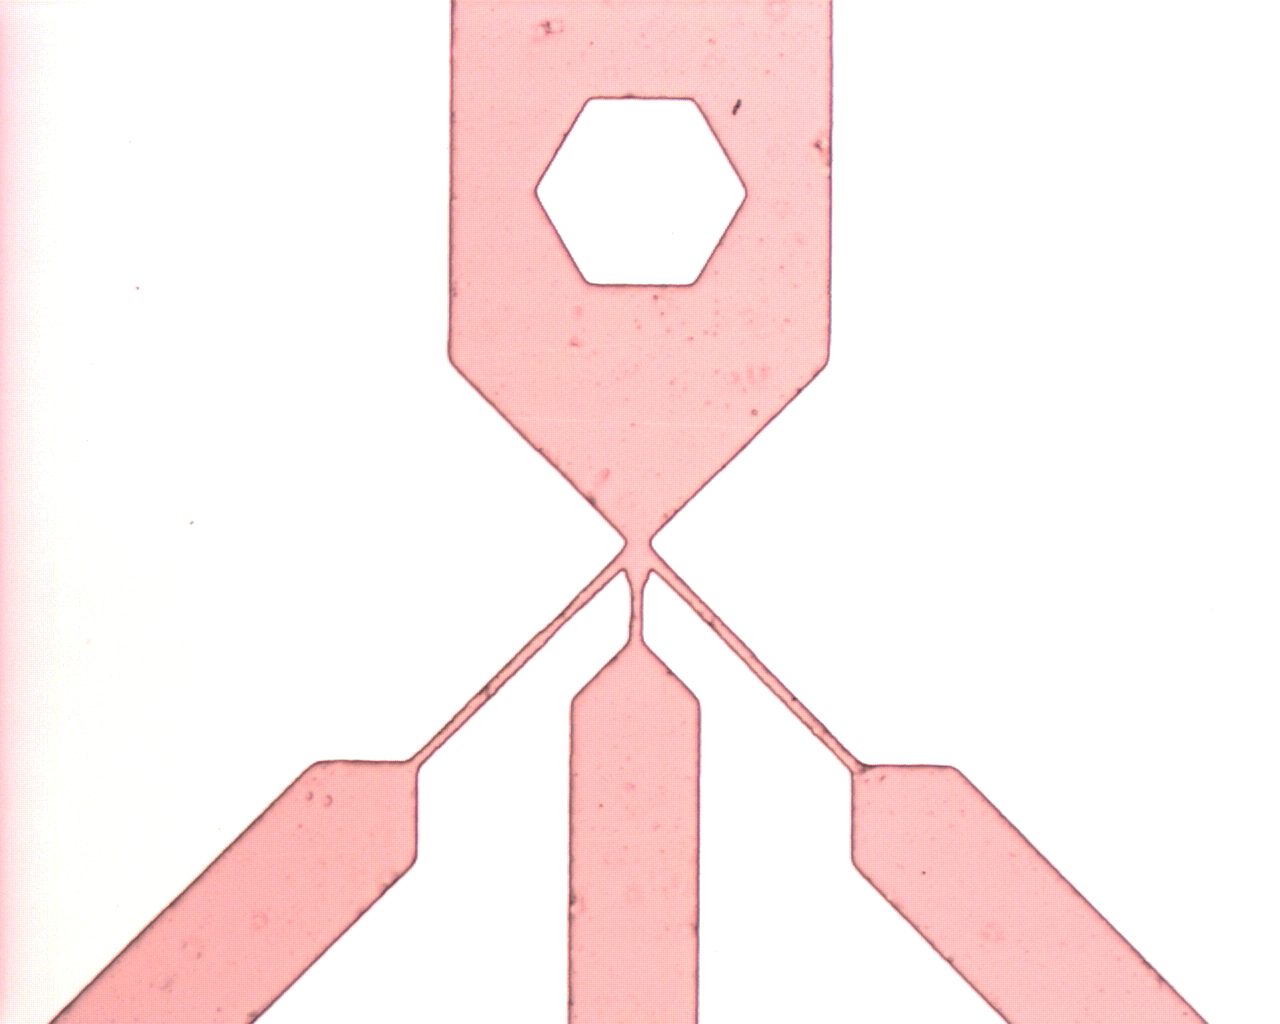
\includegraphics[width=0.7\textwidth]{images/su8_results.png}
    \caption{SU-8 photoresist as the master mold for PDMS micro-fluidic channels.}
    \label{fig:su8_results}
\end{figure}

\par The SU-8 master mold created through photolithography with the transparency mask, matched the transparency and the designed mold height closely. A representative SU-8 mold is depicted in figure \ref{fig:su8_results}. The dimensions of the SU-8 mold was verified using the Ambios Xp-1 profilometer. The SU-8 surface profile measured by the profilometer are presented in figure \ref{fig:profilometer_300um_channel} and \ref{fig:profilometer_10um_channel_100um_sideways}. 


\begin{figure}[H]
    \centering
    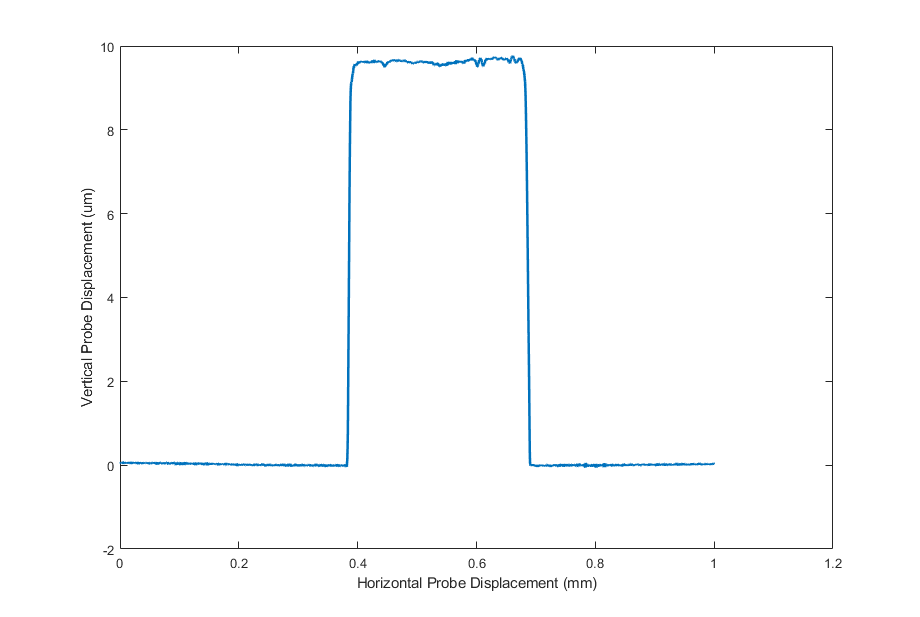
\includegraphics[width=0.8\textwidth]{images/300umWideChannel.png}
    \caption[Surface profile of a 300 micron wide channel on the SU-8 master mold.]{Surface profile of a 300 micron wide channel on the SU-8 master mold. The profile was captured with the Ambios XP-1 profilometer. The profilometer recorded a channel height of 9.6 microns.}
    \label{fig:profilometer_300um_channel}
\end{figure}

\begin{figure}[h]
    \centering
    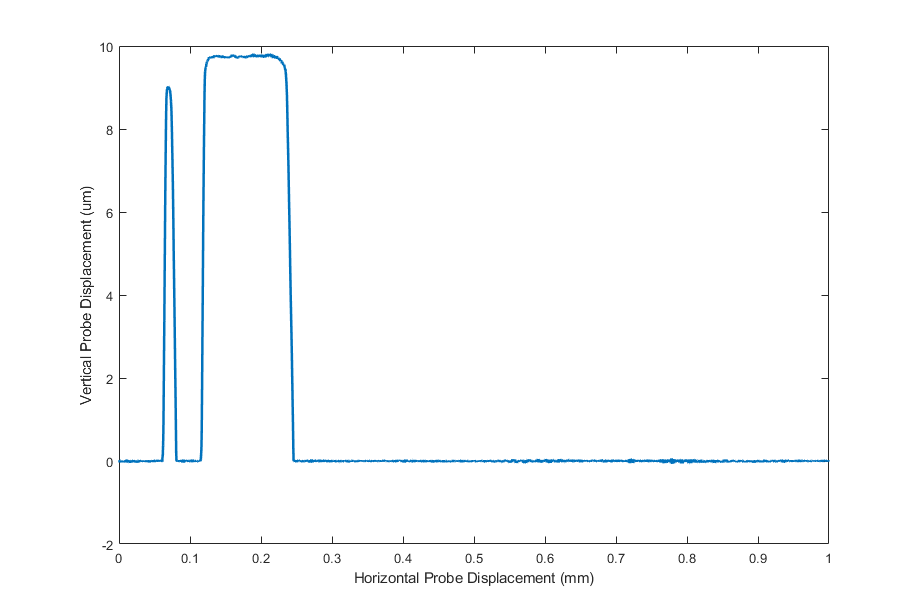
\includegraphics[width=0.8\textwidth]{images/10umWideAndSidewaysThrough100umWide.png}
    \caption[Surface profile of a 10 micron and 100 micron wide channel on the SU-8 master mold.]{Surface profile of a 10 micron and 100 micron wide channel on the SU-8 master mold. The profile was captured with the Ambios XP-1 profilometer. The data depicts the 100 micron channel as about 140 microns wide since it crossed the channel at 45$^\circ$. The profilometer recorded a channel height of 9 and 9.6 microns for the 10 micron and 100 micron channels respectively.}
    \label{fig:profilometer_10um_channel_100um_sideways}
\end{figure}

\par PDMS casts were successfully fabricated from the SU-8 molds and operation was validated by successfully plasma bonding the casts to glass blanks and verifying channel flow with no leaks or clogs. Figure \ref{fig:pdms_results} displays a typical PDMS cast.

\begin{figure}[H]
    \centering
    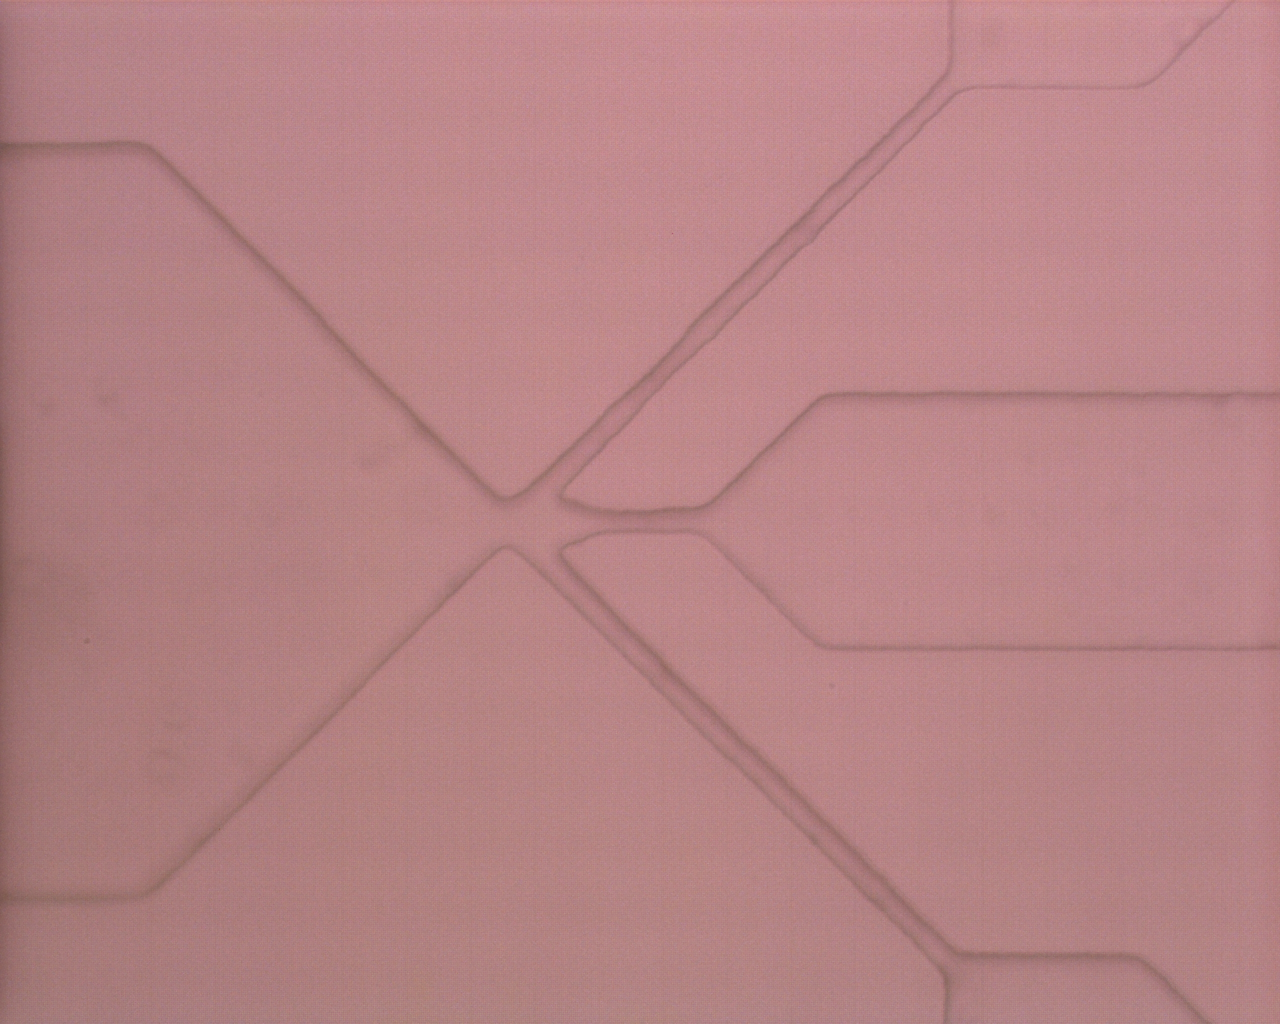
\includegraphics[width=0.7\textwidth]{images/PDMS_channels.png}
    \caption{PDMS cast from the master mold. Once bonded to a glass substrate, the cast will form the micro-fluidic channels of the device.}
    \label{fig:pdms_results}
\end{figure}

\FloatBarrier


\subsection{Electrode Fabrication}

\par The micro-electrode fabrication process was developed with Dr. Ben Hawkins and Jack Foley through the course of this thesis. The fabrication process was developed with an iterative approach of tuning process parameters and was met with many failures.

\begin{figure}[h]
    \centering
    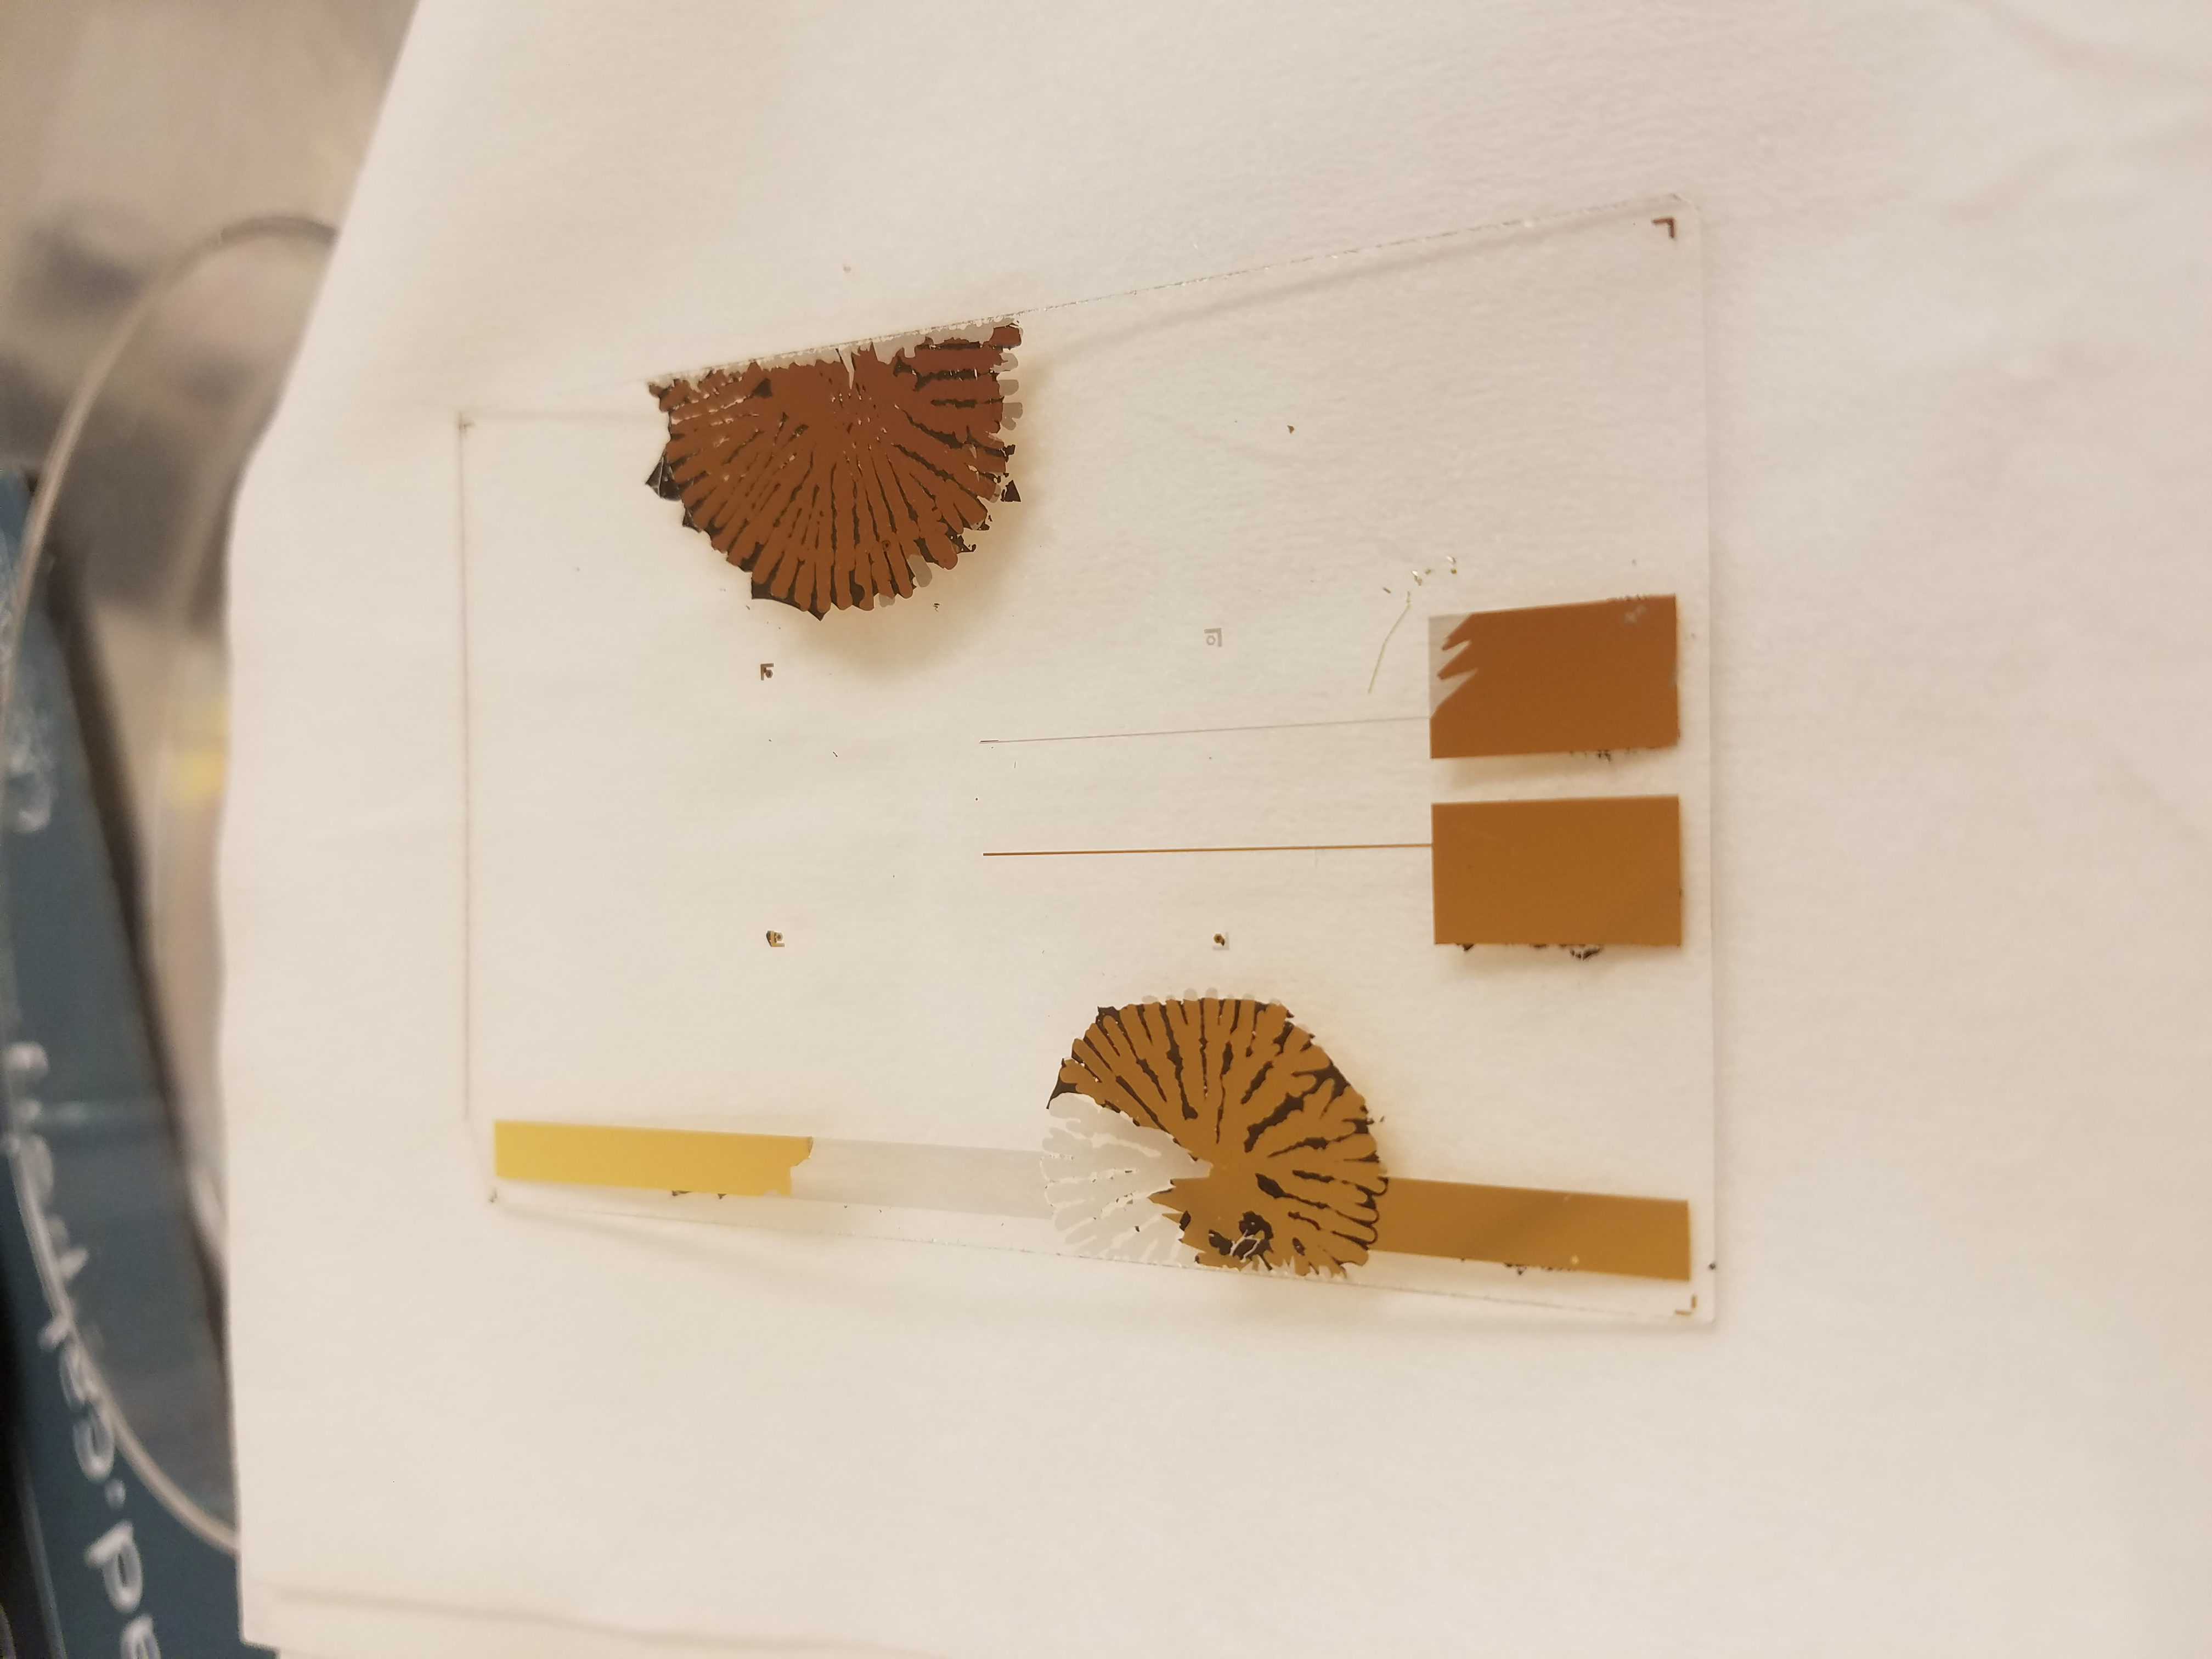
\includegraphics[width=\textwidth]{images/adhesion_issues.jpg}
    \caption{Electrode fabrication failure demonstrating two modes of failure: the Ma-N1420 photoresist failed to properly adhere to the glass surface manifesting as two anomalous flower patterns, and poor adhesion of the deposited gold to the first chrome layer as evident by gold-stripped leads.}
    \label{fig:failed_electrode_macro}
\end{figure}

\par Once the photolithography process was tuned, processed electrodes were met with three main modes of failure: poor photoresist adhesion, poor gold adhesion, and thin cracks or scrapes. Figure \ref{fig:failed_electrode_macro} and \ref{fig:failed_elecftrodes_micro}  depict these failure modes at macro and micro scales respectively.

\begin{figure}[h]
    \centering
    \begin{subfigure}[t]{0.45\textwidth}
        \centering
        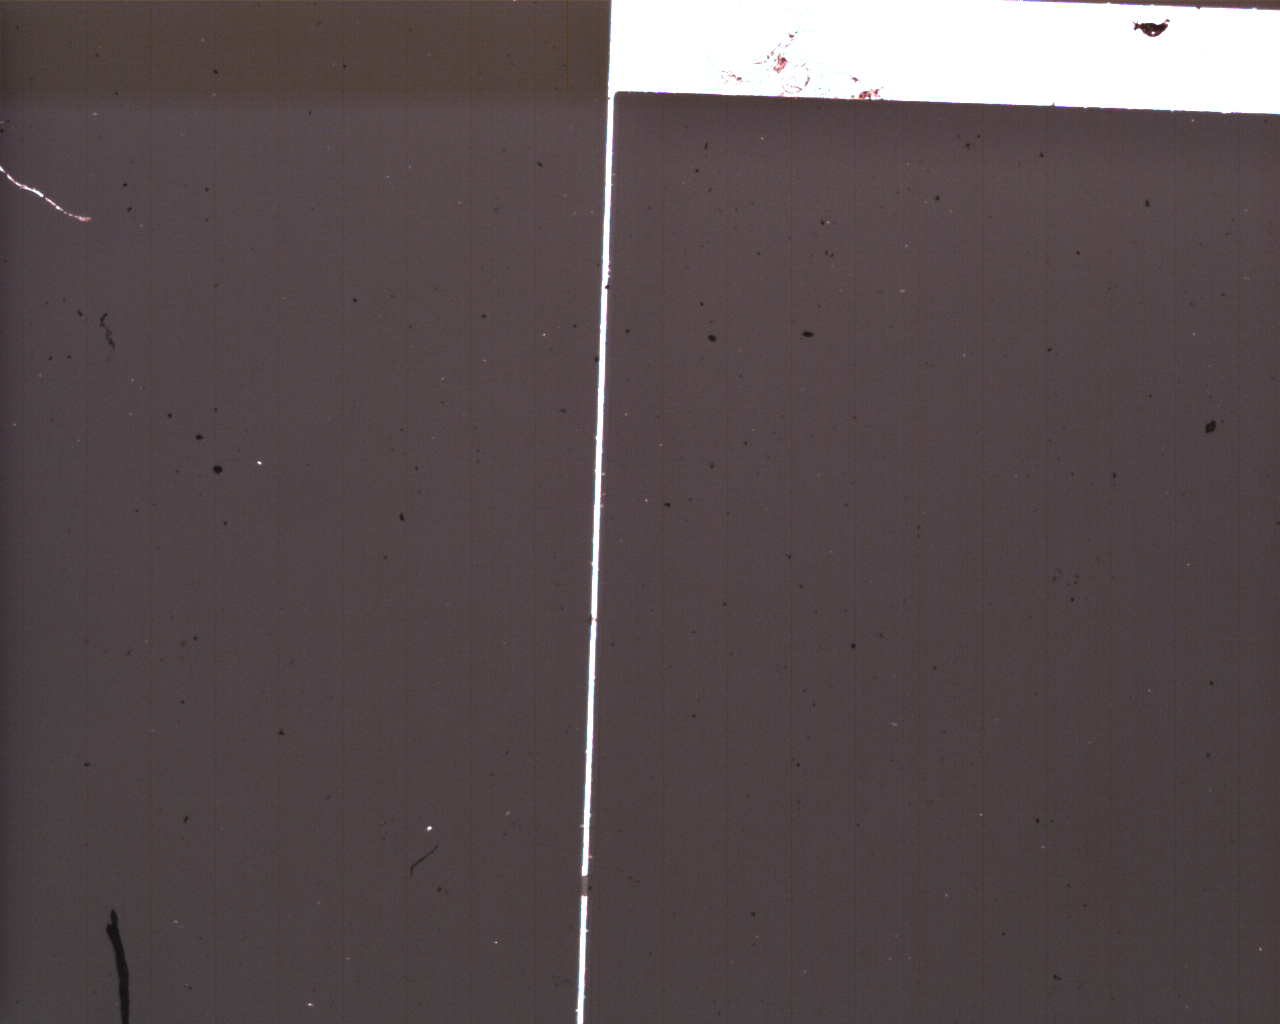
\includegraphics[width=\textwidth]{images/electrodeFailureChunkBreak.png}
        \caption{Break in electrode due to delamination of gold strip.}
    \end{subfigure}
    \hfill
    \begin{subfigure}[t]{0.45\textwidth}
        \centering
        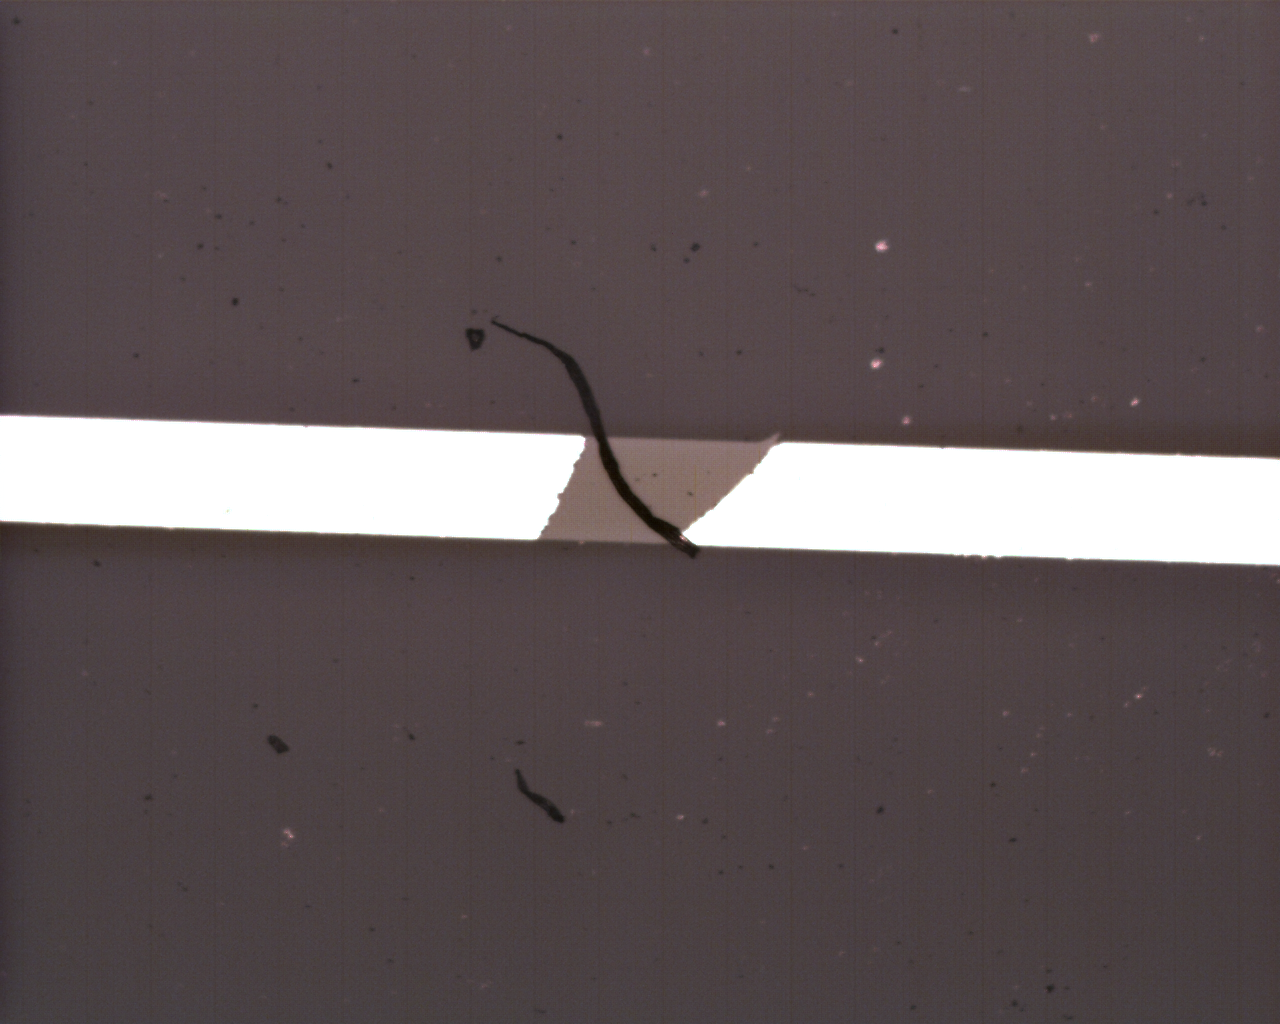
\includegraphics[width=\textwidth]{images/electrodeFailureChunkBreakZoomed.png}
        \caption{Visible chromium layer at site of electrode delamination highlights failure of gold adhesion to chromium layer.}
    \end{subfigure}
    \\
    \vspace{0.1 in}
    \begin{subfigure}[t]{0.45\textwidth}
        \centering
        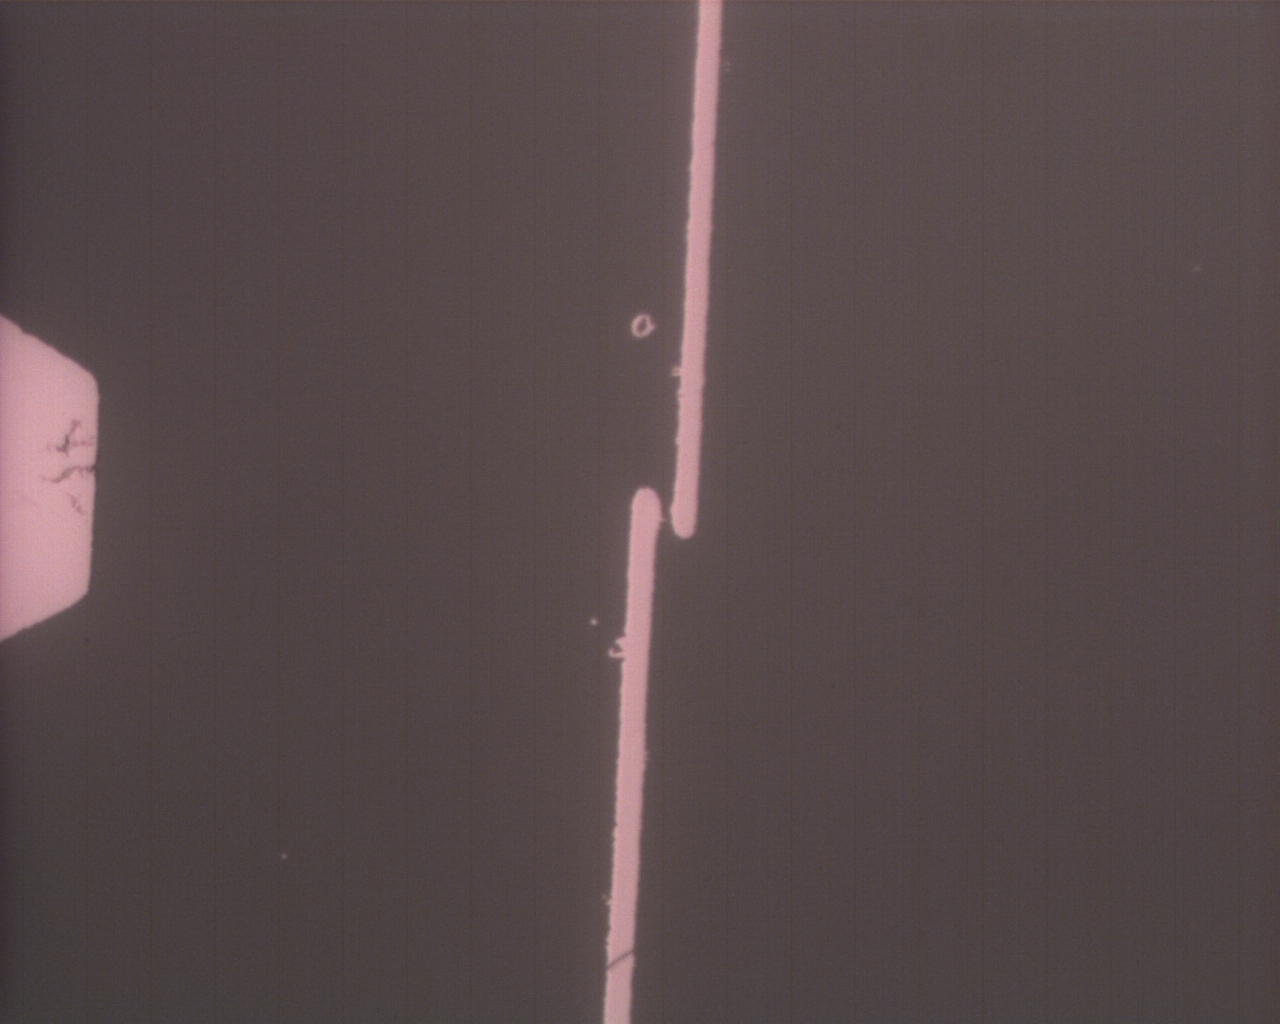
\includegraphics[width=\textwidth]{images/electrodeFailureThinBreak.png}
        \caption{Thin crack in electrode and gold.}
    \end{subfigure}
    \hfill
    \begin{subfigure}[t]{0.45\textwidth}
        \centering
        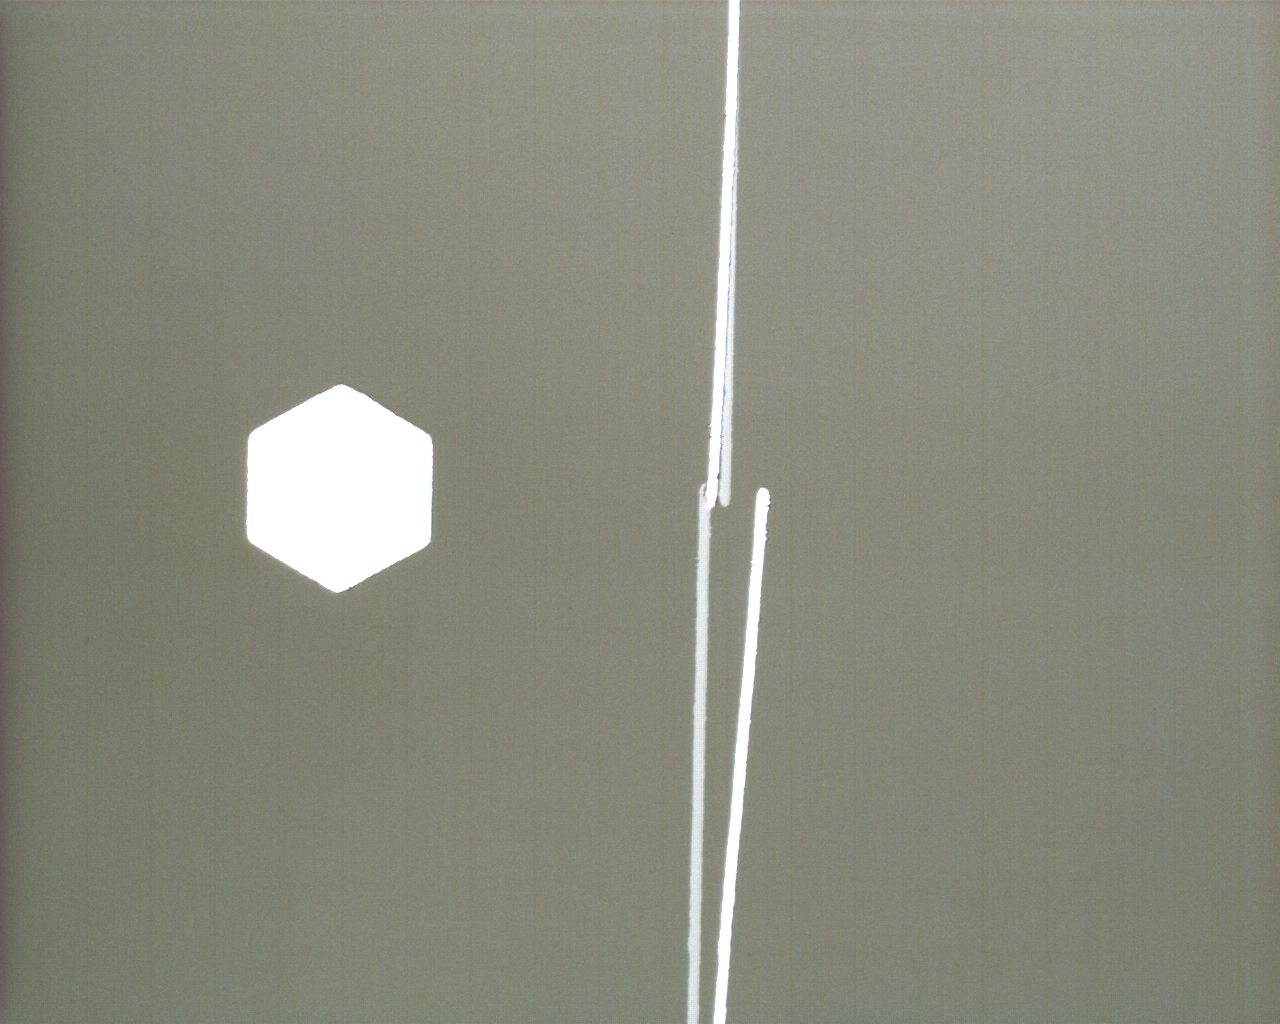
\includegraphics[width=\textwidth]{images/electrodeFailureSlide.png}
        \caption{Gold electrode strips sliding off chrome adhesion layer}
    \end{subfigure}
    \caption{Images of common electrode fabrication failures.}
    \label{fig:failed_elecftrodes_micro}
\end{figure}

\par The poor durability of the electrodes was attributed to an overall ineffectiveness of the chromium adhesion layer meant to glue the gold to the glass substrate. The process step of transferring the chromium sputtered wafer from the CrC-150 to the Denton Desk 5 sputtering system for gold deposition was identified as a likely candidate for the poor chromium-gold adhesion and hypothesized that the formation of chromium oxide during the wafer's exposure to atmosphere was the poor-adhesion culprit. In a short-term fix, the wafers were held in vacuum until they were quickly transported to the Denton Desk 5. Future microelectrode fabrication processes should take advantage of a dual-target sputtering system that can sputter chromium and gold in series while maintaining vacuum.  

\par With a remedied procedure, two additional sets of electrodes were fabricated. Figure \ref{fig:good_electrodes} depicts representative fabrication results. Overall, both sets of electrodes appeared with no initially visible cracking or delamination. However, as discussed in the following section, a set of electrodes still had adhesion issues and we only successfully fabricated one viable set of electrodes.

\begin{figure}[h]
    \begin{subfigure}[b]{\textwidth}
        \centering
        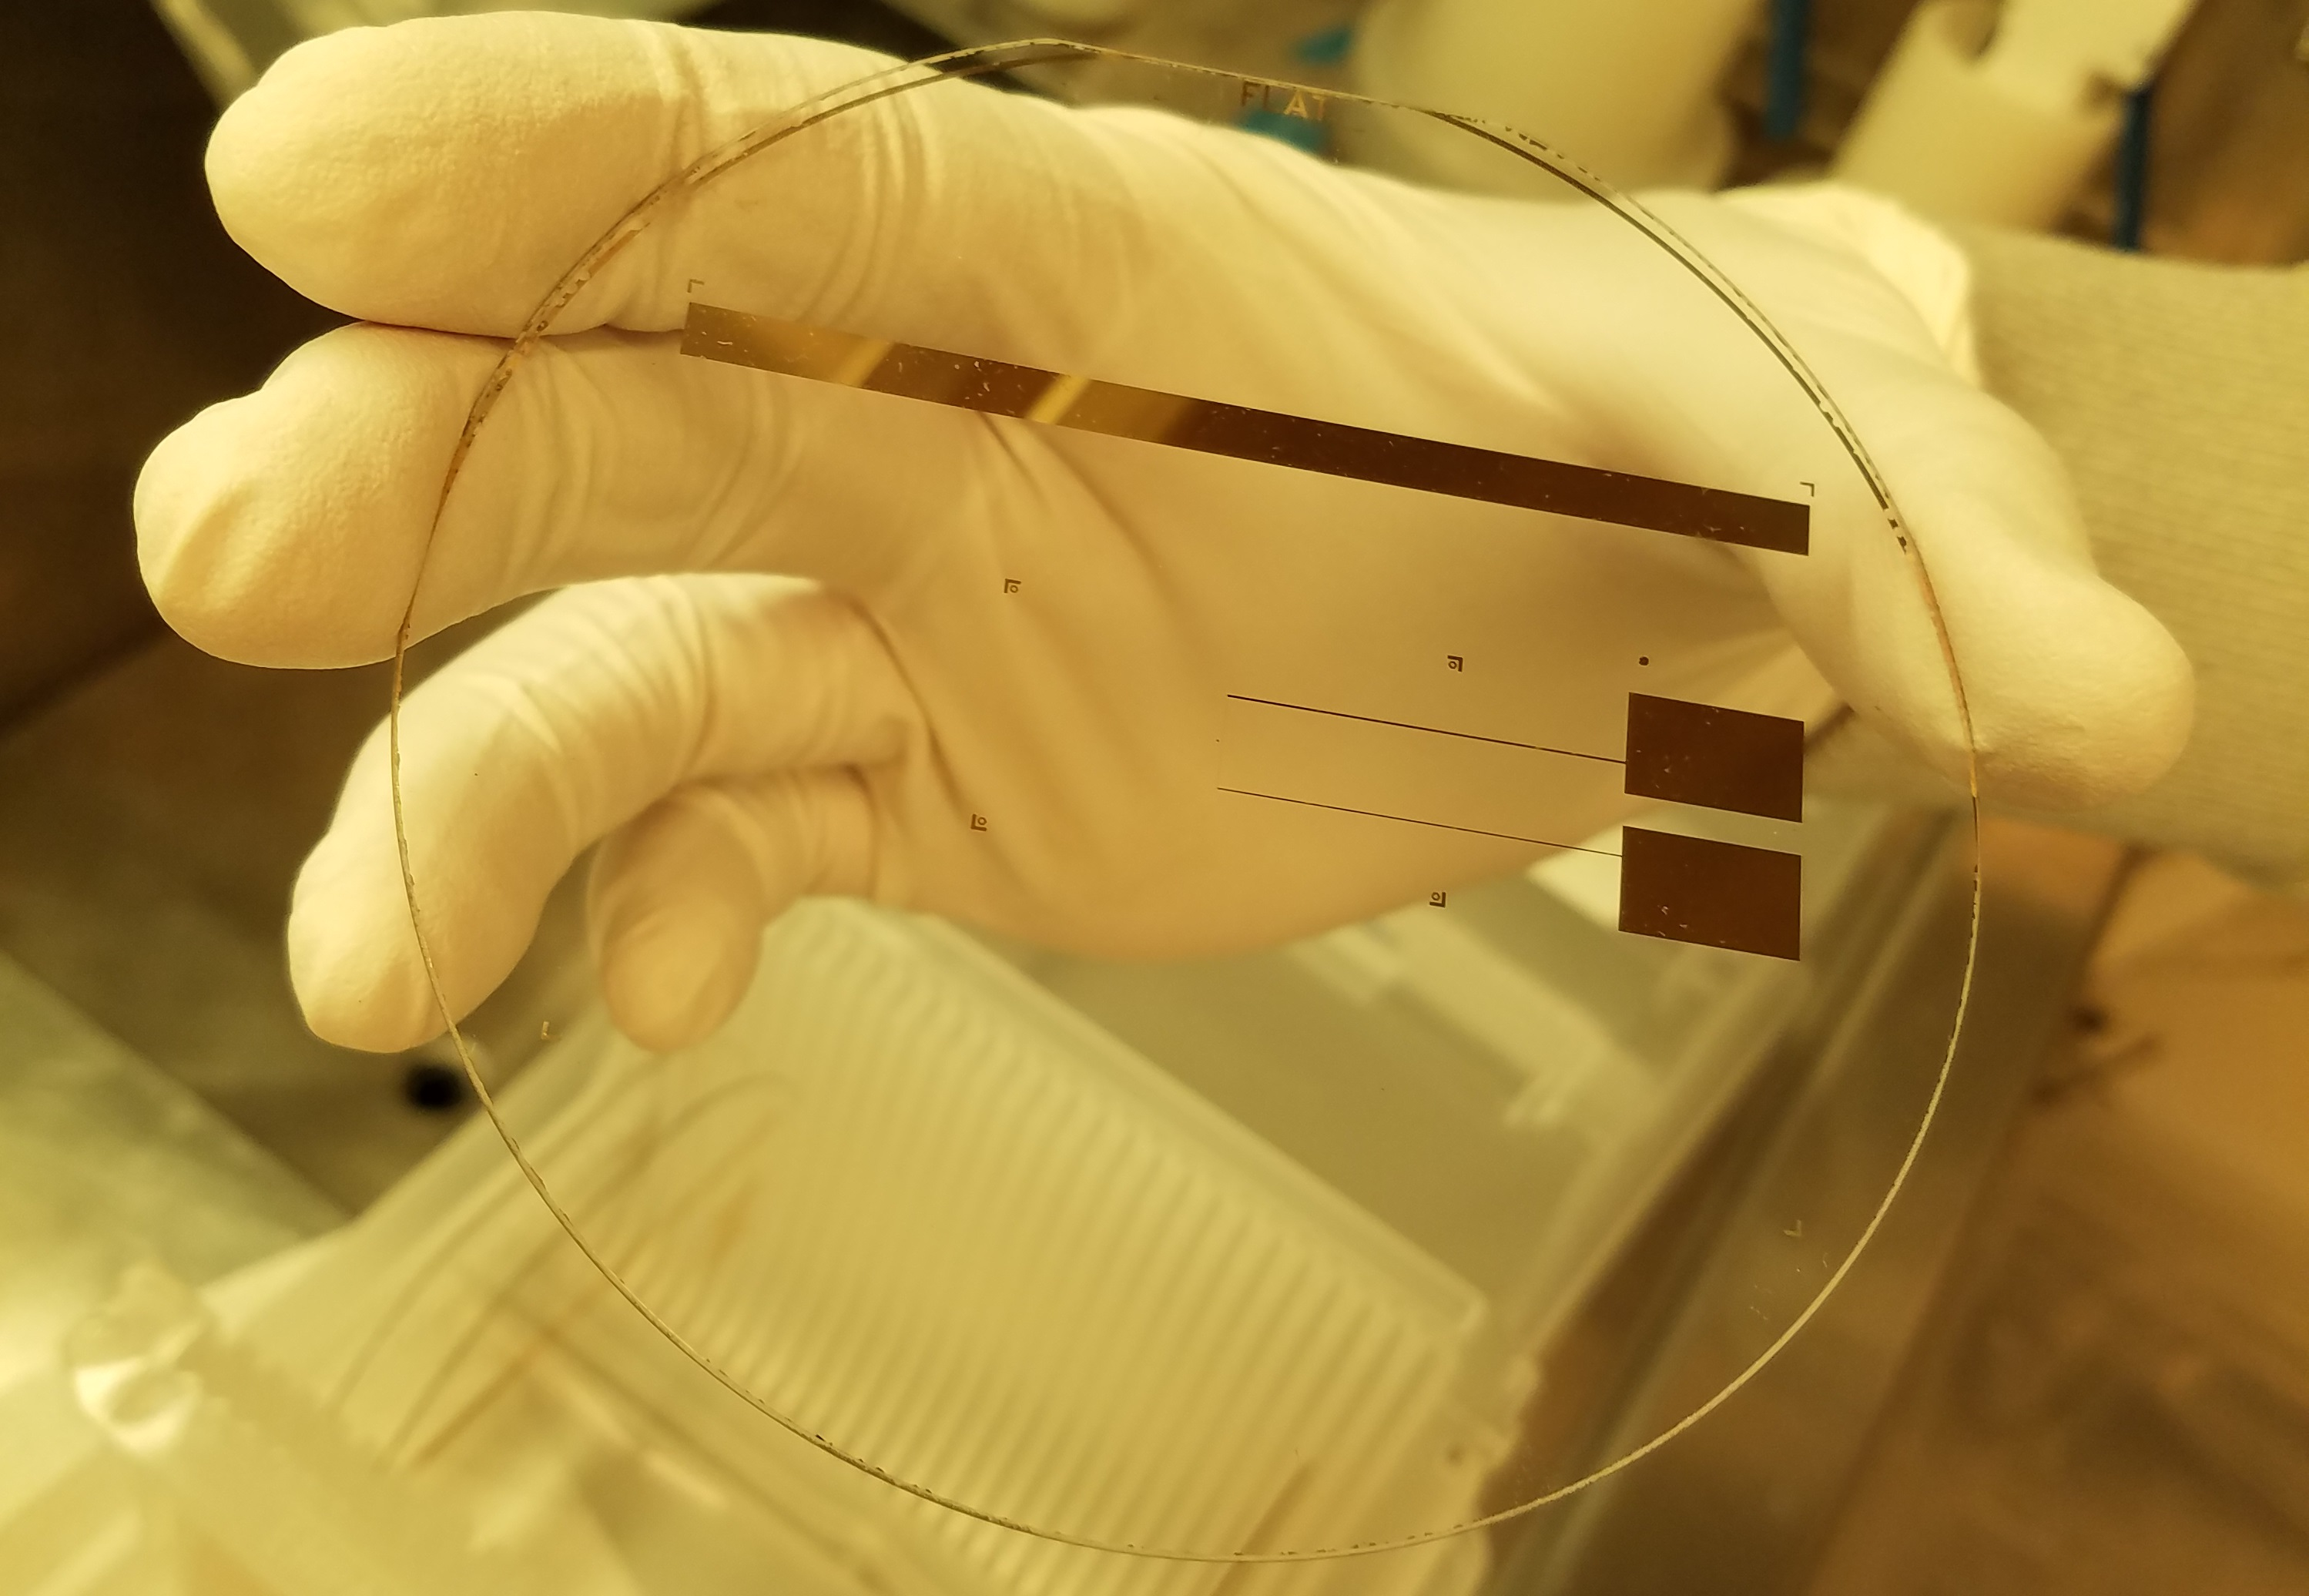
\includegraphics[width=\textwidth]{images/electrodes_real.jpg}
        \caption{Successful fabrication of device electrodes.}
    \end{subfigure}
    \\
    \vspace{0.1 in}
    \centering
    \begin{subfigure}[b]{0.45\textwidth}
        \centering
        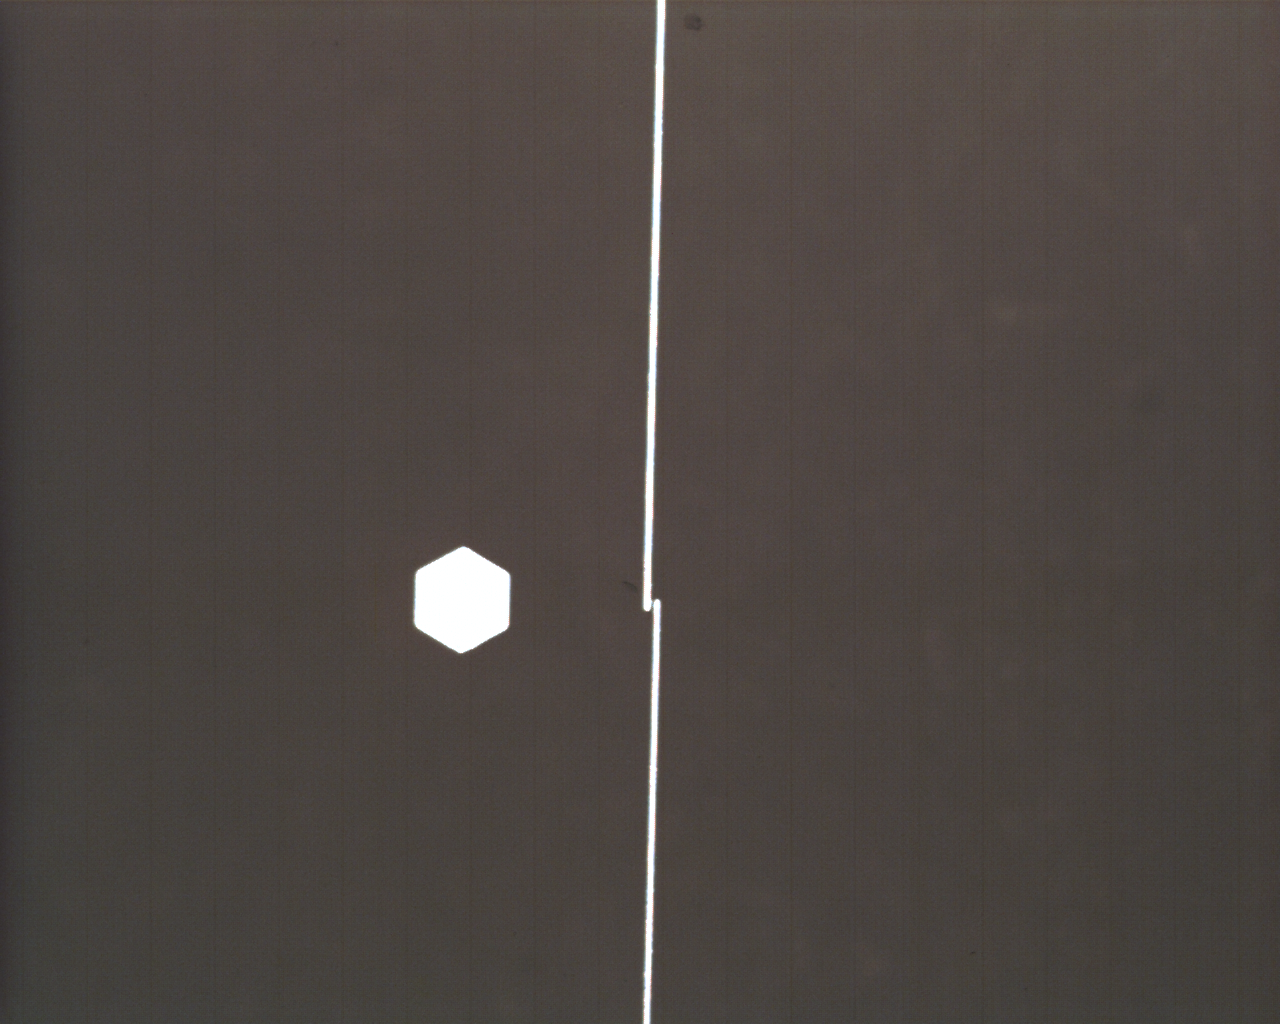
\includegraphics[width=\textwidth]{images/goodElectrode.png}
        \caption{Integral crack-prone segment.}
    \end{subfigure}
    \hfill
    \begin{subfigure}[b]{0.45\textwidth}
        \centering
        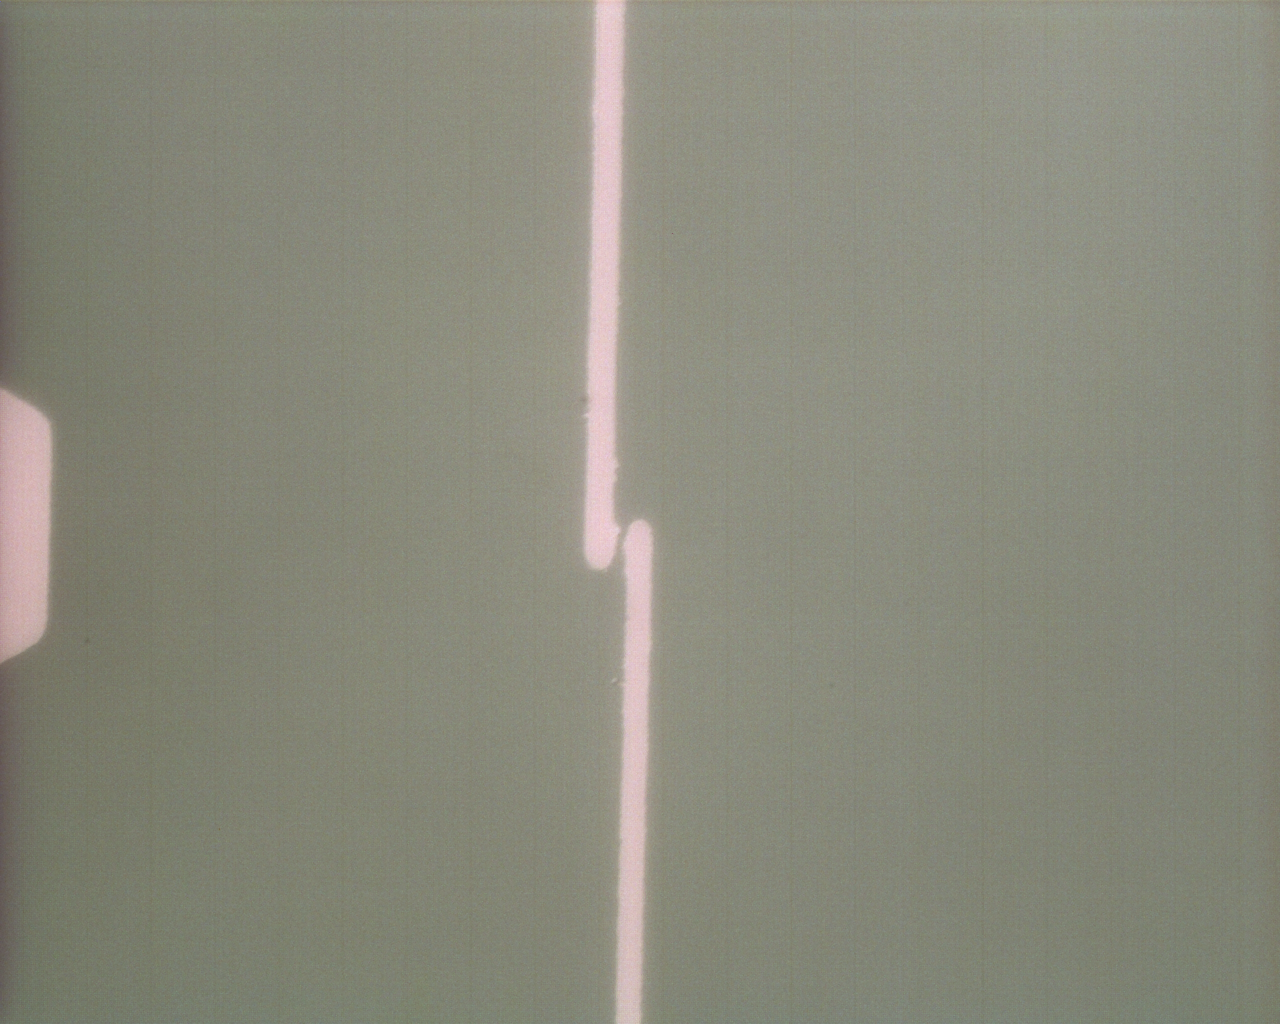
\includegraphics[width=\textwidth]{images/goodElectrodeCloseUp.png}
        \caption{Image of the electrode gap.}
    \end{subfigure}
    \caption{Integral electrodes with no breaks in sputtered gold layer. The successful results were realized by minimizing the exposure of the chromium adhesion layer to air and reducing the formation chromium oxide.}
    \label{fig:good_electrodes}
\end{figure}


\FloatBarrier

\subsection{Device Bonding}

\par By the end of the electrode fabrication process, we had what appeared like two well-adhered and integral electrode chips. Alignment for bonding was completed by hand. The first attempt of device alignment resulted in delamination of gold from the chromium adhesion layer. Although non-functional, the bonding process for the device was continued to completion. The result of the alignment and bonding is depicted figure \ref{fig:bad_device}. The device exhibited good glass-PDMS adhesion, and was later used to test microfluidics operations and particle capture with good results.

\begin{figure}[h]
    \centering
    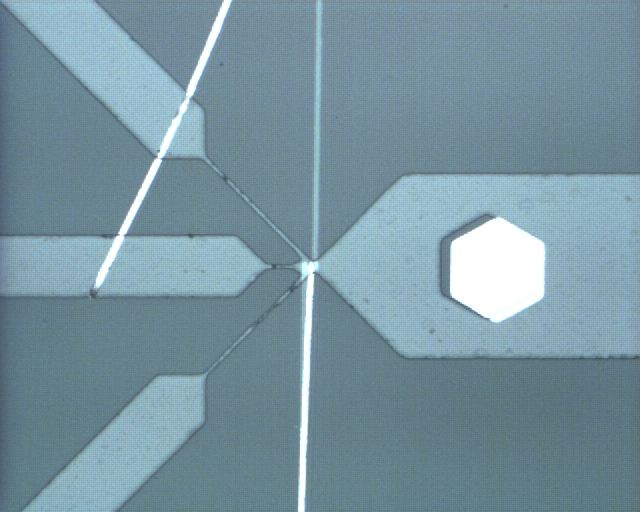
\includegraphics[width=\textwidth]{images/bad_device.png}
    \caption{Electrode adhesion failure during plasma bonding process of device 1. The sputtered gold layer delaminated from the chromium adhesion layer during PDMS to electrode alignment.}
    \label{fig:bad_device}
\end{figure}

\par The second attempt resulted in a successful alignment and bonding. Figure \ref{fig:good_device} displays the alignment and bonding results for device 2. There is a rotational device misalignment, but is centered on the sensor chamber where the electrodes are nearly perfectly aligned. This rotational misalignment is expected to have no effect on the recorded impedance spectra. The electrodes survived the alignment process with no delamination or cracks. Plasma bonding produced  strong PDMS-glass adhesion. 

\begin{figure}[h]
    \centering
    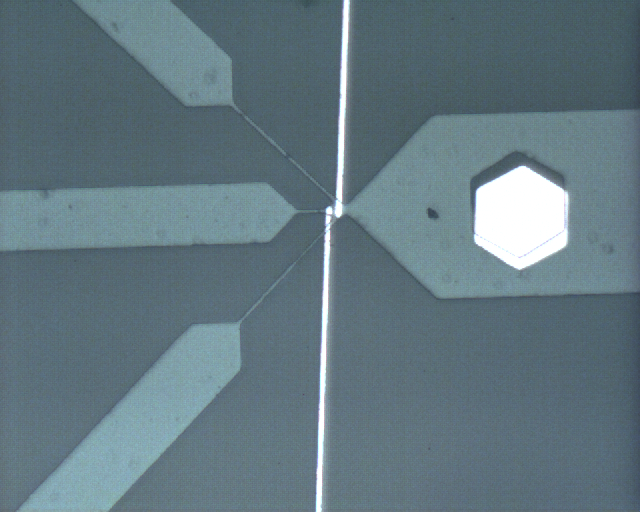
\includegraphics[width=\textwidth]{images/good_device.png}
    \caption{Successfully bonded impedance spectroscopy device. PDMS and electrodes were aligned by hand. There is a slight rotational misalignment, but should be functionally negligible.}
    \label{fig:good_device}
\end{figure}

\par The micro-fabrication results gave us one viable impedance spectroscopy device, and a procedure for creating new viable chips.

\FloatBarrier

\section{Impedance Spectroscopy System}

\par To characterize and evaluate the impedance spectroscopy system, the microfluidic performance of the IS chip was evaluated, the impedance spectroscopy measurement system was validated, and the performance of impedance spectroscopy with the IS chip was analyzed. 

\subsection{Microfluidic Performance Evaluation}

\par As expected and discussed in chapter \ref{ch: introduction}, the current microfluidic design is not capable of isolating a single cell. This is largely due to the tolerances of the transparency masks as discussed in section \ref{sec:PDMS_cast_fabrication}. However, the device was evaluated on its ability to flow solutions, saturate the sensor chamber with beads, and clear the sensor chamber of beads. See figure \ref{fig:assembled_good_device} for the fully assembled impedance spectroscopy chip under testing. 

\begin{figure}[h]
    \centering
    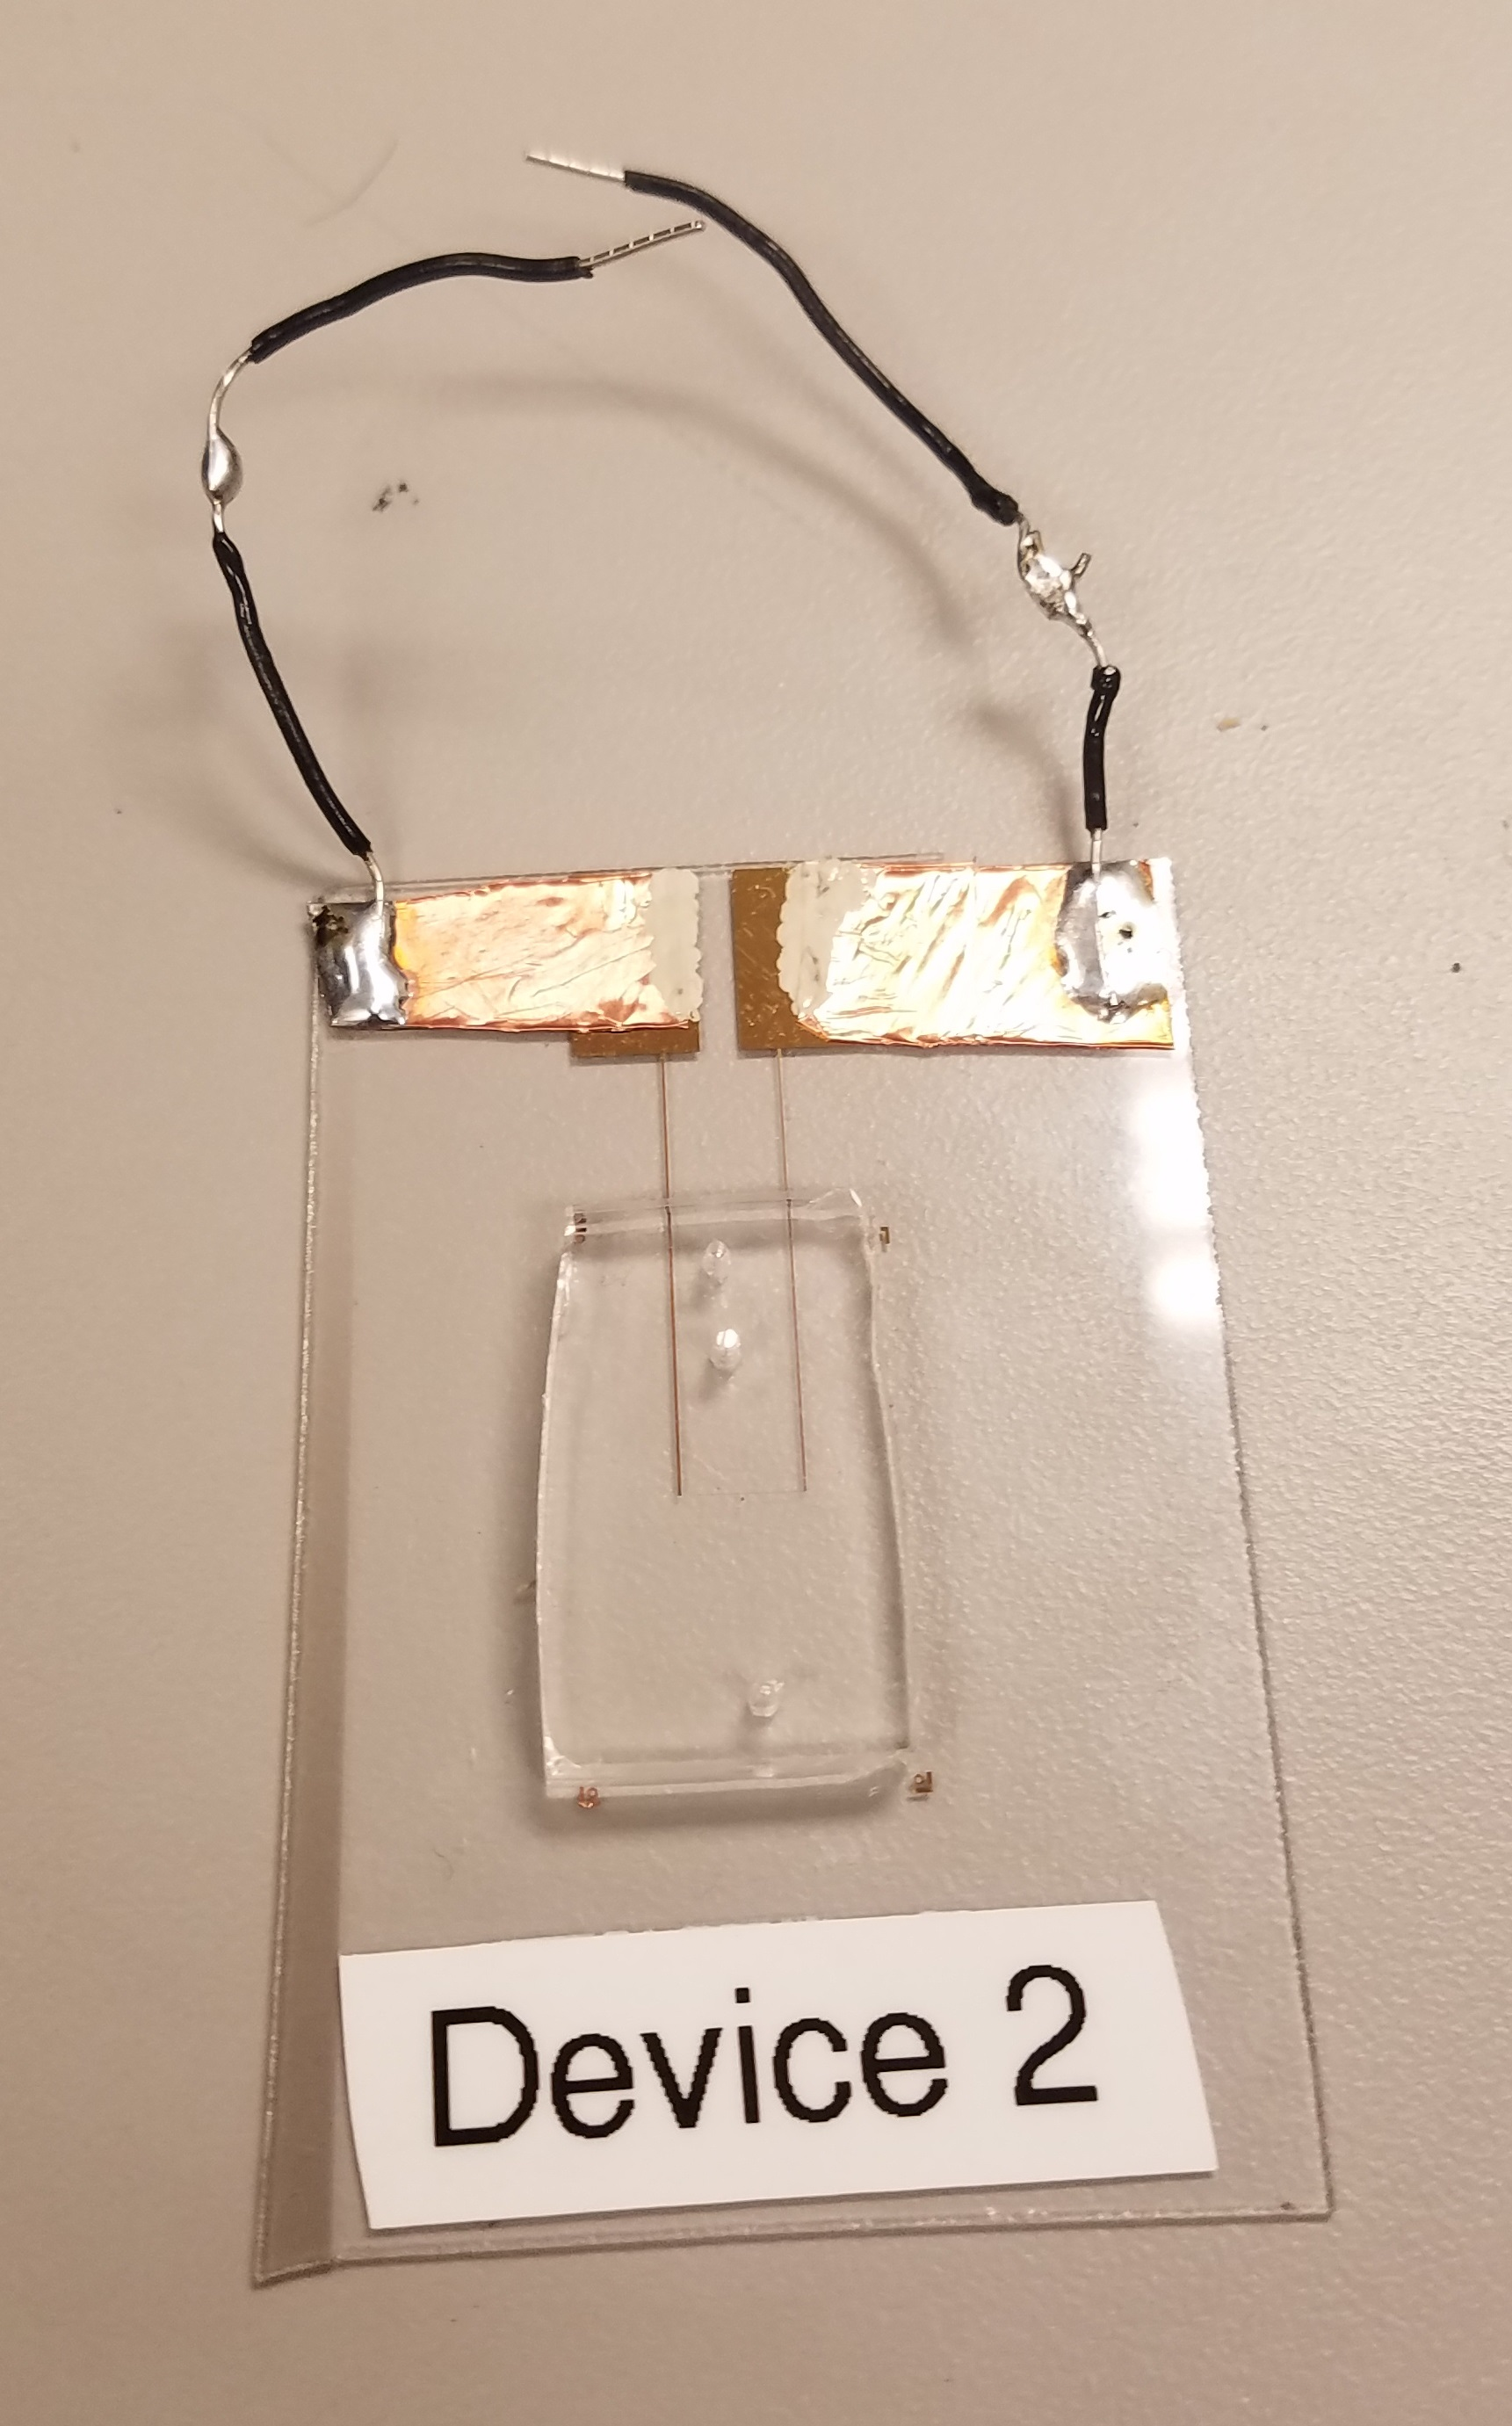
\includegraphics[width=0.5\textwidth]{images/device_22.jpg}
    \caption{Successfully assembled cell impedance spectroscopy device.}
    \label{fig:assembled_good_device}
\end{figure}

\par Using the the Harvard Apparatus syringe pumps, PBS and DI water were successfully pumped into impedance spectroscopy chip. However, the introduction of 7 $\mu$m polystyrene beads initiated debris flow. With a careful application of alternating flow, we succeeded in saturating and flushing the sensor region of polystyrene beads over several days. The device was ultimately jammed and delaminated under applied pressure.

\begin{figure}[h]
    \centering
    \begin{subfigure}[b]{0.45\textwidth}
        \centering
        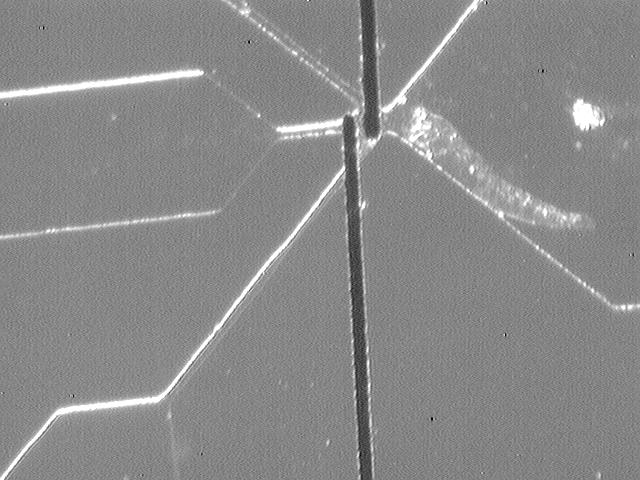
\includegraphics[width=\textwidth]{images/IS_empty.jpg}
        \caption{Sensor chamber saturated with phosphate buffered solution.}
    \end{subfigure}
    \hfill
    \begin{subfigure}[b]{0.45\textwidth}
        \centering
        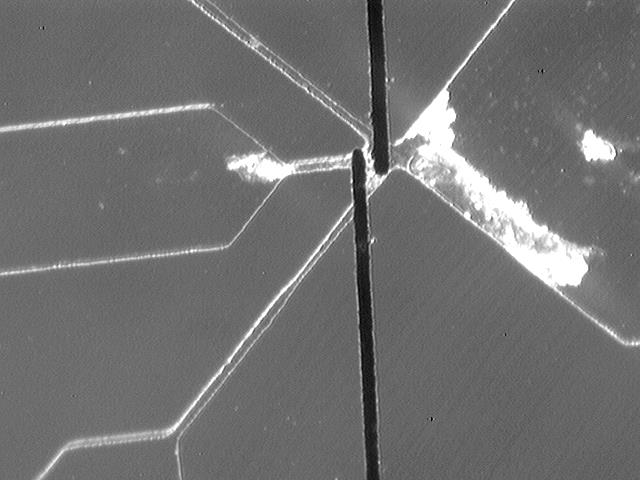
\includegraphics[width=\textwidth]{images/IS_particle_saturation.jpg}
        \caption{Sensor chamber saturated with 7$\mu$m polystyrene beads.}
    \end{subfigure}
    \\
    \vspace{0.1 in}
    \begin{subfigure}[b]{0.45\textwidth}
        \centering
        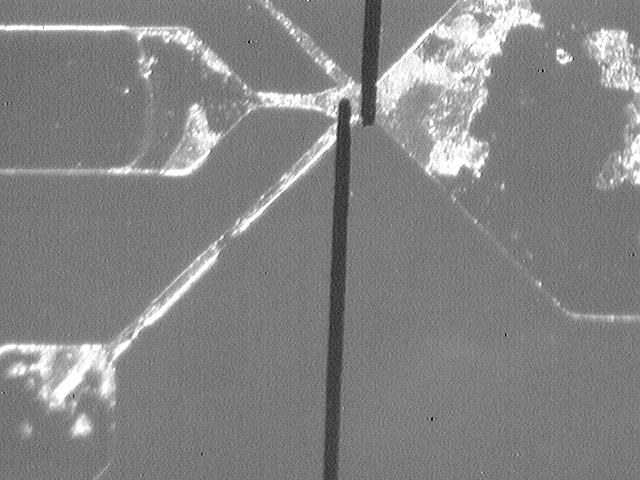
\includegraphics[width=\textwidth]{images/IS_jammed.jpg}
        \caption{Sensor region jammed with debris and beads.}
    \end{subfigure}
    \hfill
    \begin{subfigure}[b]{0.45\textwidth}
        \centering
        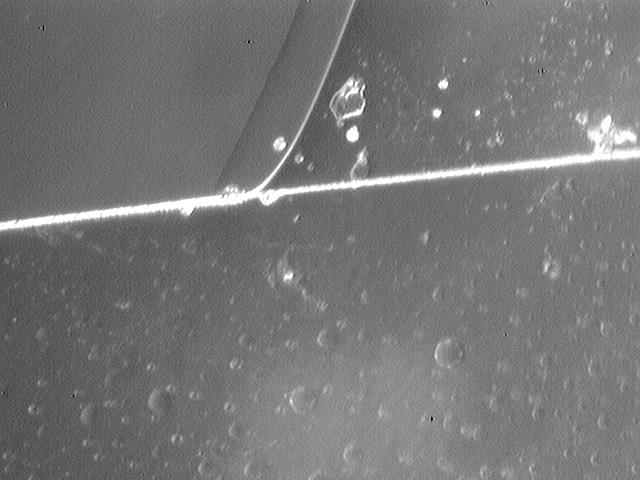
\includegraphics[width=\textwidth]{images/IS_device_delamination.jpg}
        \caption{Device delaminated after attempt to flush jammed sensor region.}
    \end{subfigure}
    \caption{Images of the sensor region of the impedance spectroscopy device. The device successfully measured fluid and 7 $\mu$m beads before the sensor region became jammed and the device ultimately delaminated. Images were taken with the LabSmith SVM340 inverted microscope.}
    \label{fig:IS_sensor_reigon_measurement}
\end{figure}

\par Fortunately, a sizable, but limited, body of data was collected. The following section describes the collected data and characterizes the device response to deionized water, phosphate buffered solution, and a suspension of polystyrene beads.

\FloatBarrier


\clearpage

\subsection{Impedance Spectroscopy Measurement System Validation}

\par The validation of the impedance spectroscopy system focused on the data acquisition system and the impedance calculating circuit. Operation utilizing the cell impedance chip was reserved for the following section.

\begin{figure}[h]
\centering
    \begin{subfigure}[b]{\textwidth}
        \centering
        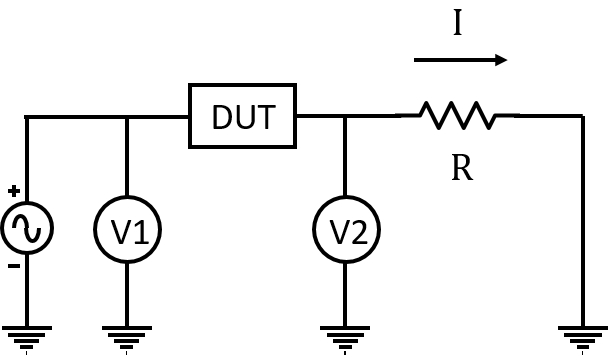
\includegraphics[width=0.5\textwidth]{images/I-VMethod.png}
        \caption{The idealized test circuit.}
        \label{fig:IS_DAQ_test_circuit_ideal}
    \end{subfigure}
    \\
    \vspace{0.1 in}
    \begin{subfigure}[b]{\textwidth}
        \centering
        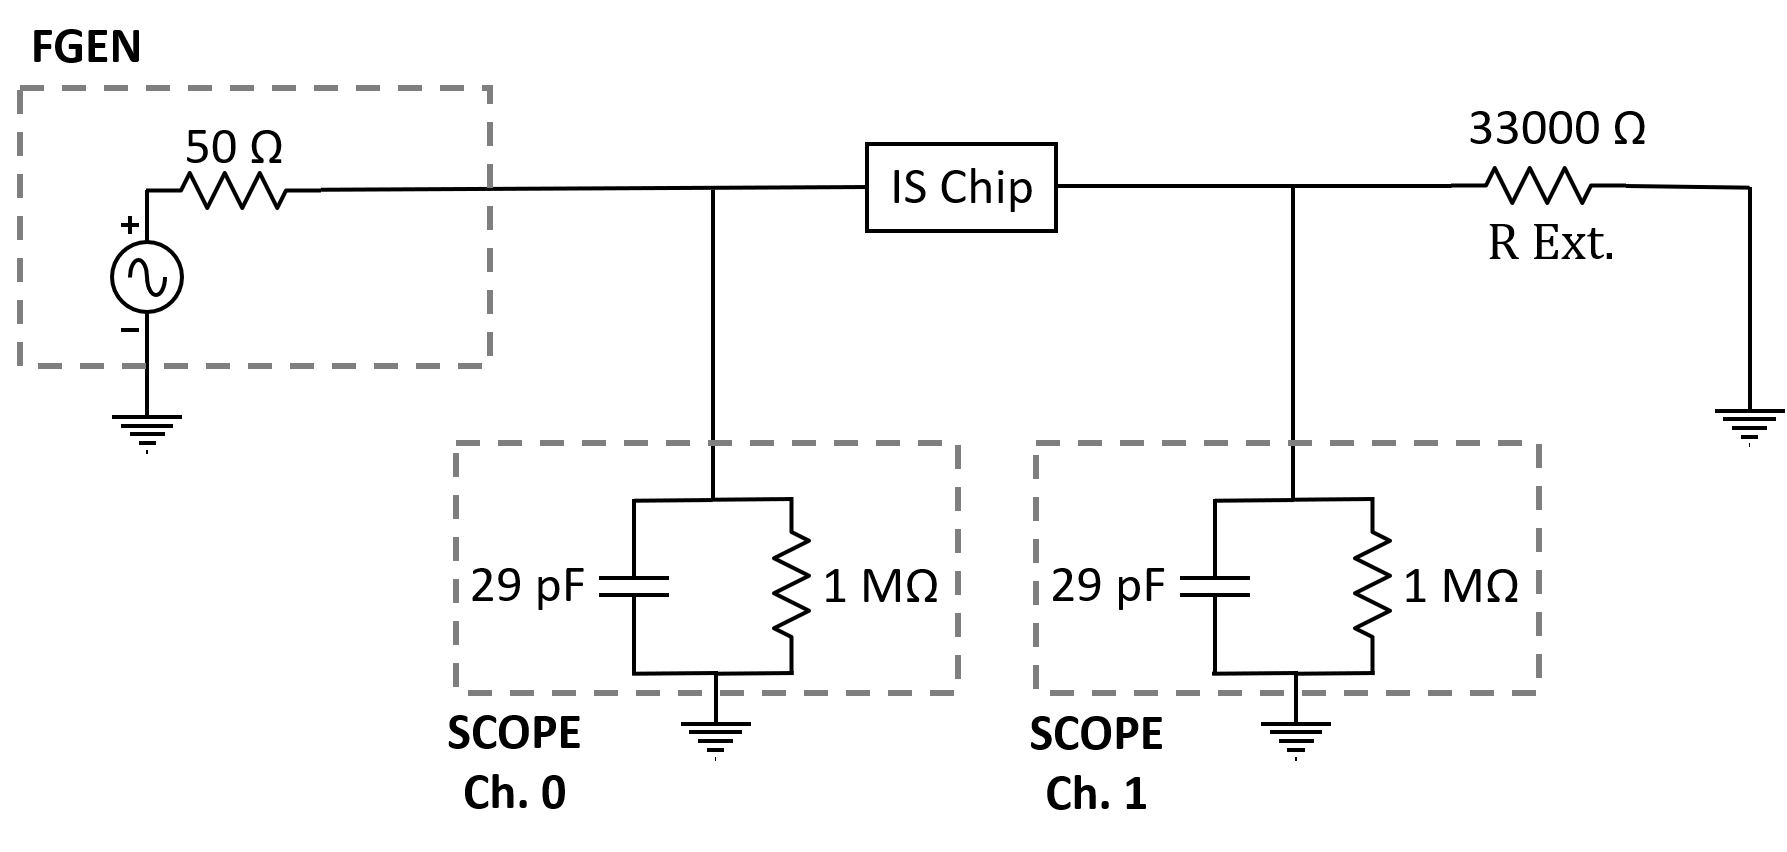
\includegraphics[width=0.9\textwidth]{images/method_I-V.png}
        \caption{The implemented test circuit.}
        \label{fig:IS_DAQ_test_circuit_implemented}
    \end{subfigure}
    \caption{The idealized and implemented I-V circuits. For the validation tests, a 10 pF capacitor was used in place of the IS chip or DUT, and a 33 k$\Omega$ resistor was used as the external resistor.}
    \label{fig:IS_DAQ_test_circuit}
\end{figure}

\par To validate and investigate the impedance spectroscopy DAQ system, the test circuit in figure \ref{fig:IS_DAQ_test_circuit_implemented} was physically implemented and tested with the IS system. The results were compared to simulations of the implemented circuit and the ideal circuit in figure \ref{fig:IS_DAQ_test_circuit_ideal}. A 10 pF capacitor was used as the device under testing. The use of the capacitor was justified by noting that the electric double layer will be the largest impedance contributor, and using Gongadze's experimentally determined EDL capacitance of 6$\mu$F/cm$^2$ for titanium electrodes \cite{_gongadze.pdf_????}, and assuming each electrode has a fluid contact area of 11.5 $\mu$m by 15 $\mu$m, the capacitance of the EDL for our electrodes can be very roughly estimated as 5.2 pF. Using a capacitor of 10 pF as the DUT is well within the margin of error.  

\par As illustrated in the bode plot of figure \ref{fig:test_circuit_bode}, the measured data and the implemented circuit simulation with scopes largely matched, but there were large deviations from the idealized simulation. The I-V method assumes that all current flowing through the DUT is also flowing through the external resistor $R_{EXT}$, but with the application of oscilloscope 1, this is no longer the case. All current that leaks through oscilloscope 1 will inflate the calculated impedance of the DUT.  

\begin{figure}[h]
    \centering
    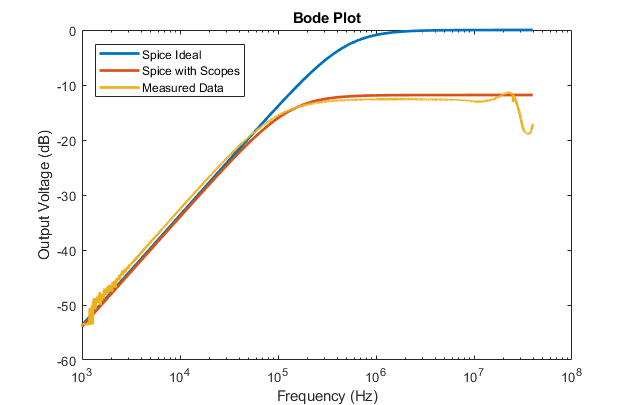
\includegraphics[width=0.9\textwidth]{images/spice-measured-comp.png}
    \caption{Bode plot of the ratio of the voltage out of the DUT to the voltage in.}
    \label{fig:test_circuit_bode}
\end{figure}

\par Revisiting the impedance solution using the I-V method, we have
\begin{equation}
    Z_{DUT} = \frac{V_1 - V_2}{I}.
\end{equation}

\noindent In ideal scenarios, we would assume all current flows through the external resistor and then $I = V_2 / R_{EXT}$. However, we know this is not true: the non-ideal properties allows current to flow through our attached oscilloscopes. This additional current flow can be compensated by replacing $R_{EXT}$ with $Z_{EXT}$ which accounts for the impedance of the oscilloscope and the external resistor. 

\begin{equation}
    Z_{DUT} = \bigg(\frac{V_1 - V_2}{V_2}\bigg)Z_{EXT}.
    \label{eqn:corrected_IV}
\end{equation}

\par Given the equivalent circuit of the oscilloscope, $Z_{EXT}$ can be expressed as

\begin{equation}
    Z_{EXT} = \bigg(jwC_{s}+\frac{1}{R_{s}}+\frac{1}{R_{EXT}}\bigg)^{-1},
    \label{eqn:corrected_Rext}
\end{equation}
\noindent where $C_{s}$ and $R_{s}$ are the capacitance and resistance of the oscilloscope respectively. For data that is calculated with the uncorrected I-V formula, the data can be corrected as follows:
\begin{equation}
    Z_{DUT} = Z_{NC}\bigg(\frac{Z_{EXT}}{R_{EXT}}\bigg),
\end{equation}
\noindent where $Z_{NC}$ is the non-corrected data. 

\par The error associated by attaching the oscilloscope can be quantified as
\begin{equation}
    \pmb{\%} \textbf{Error} = 100 \cdot \bigg| 1 - \frac{R_{EXT}}{Z_{EXT}}\bigg|.
    \label{eqn:oscilloscope_error}
\end{equation}

\par Figure \ref{fig:test_circ_measurement_error} displays the measured percent error and the error calculated from equation \ref{eqn:oscilloscope_error} due to the attached oscilloscope. Although there is a significant amount of unaccounted error in the noisy low frequencies and frequencies above 25 MHz, the error due to the attached oscilloscope appears to account for the majority of the error over the applied frequency range.

\begin{figure}[h]
    \centering
    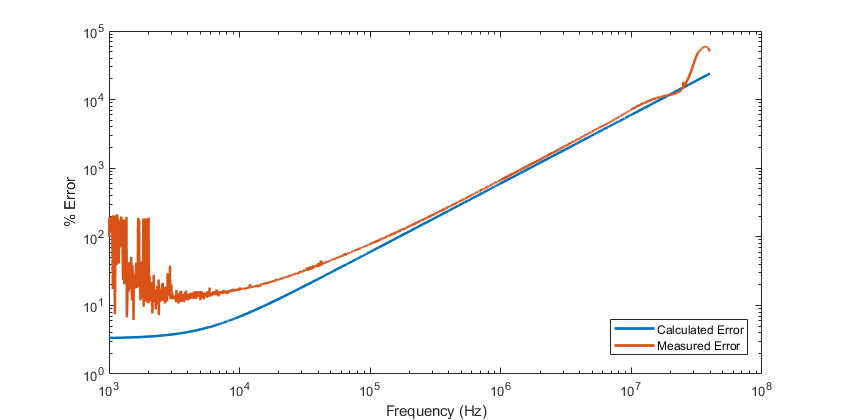
\includegraphics[width=0.85\textwidth]{images/percentError.png}
    \caption{Comparison of the calculated percent error due to the oscilloscopes and the measured percent error.}
    \label{fig:test_circ_measurement_error}
\end{figure}

\par The correction function, equation \ref{eqn:corrected_IV}, was applied to the measured data and the results are presented in figure \ref{fig:IS_validation_corrected_spectra_comp}. The residual error is displayed in figure \ref{fig:IS_residual_error}. Between 3 kHz and 25 MHz, the percent error does not increase beyond 30\%, a significant improvement over the exponential error of the uncorrected data. The unaccounted residual error may be attributed to parasitic capacitance in the breadboard and system at large; deviations in reported values in the external resistor, the oscilloscope, and the test capacitor; and high frequency parasitic inductance.

\begin{figure}[h]
\centering
\begin{subfigure}[b]{\textwidth}
    \centering
    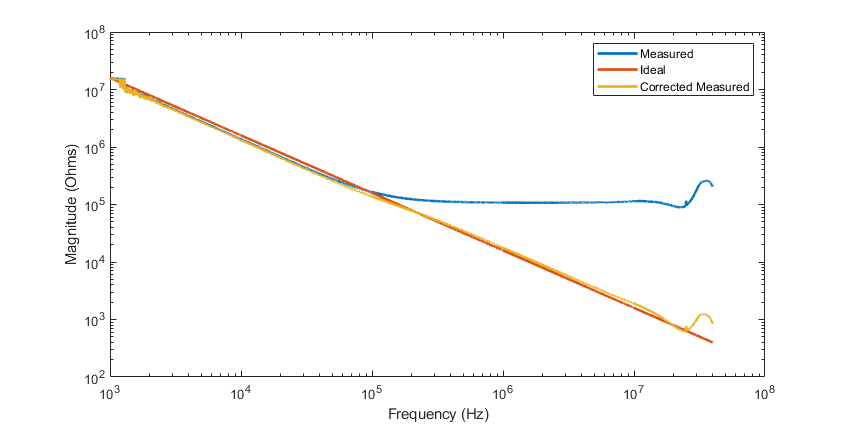
\includegraphics[width=\textwidth]{images/CorrectedImpedanceMag.png}
    \caption{Plot of the measured, ideal, and corrected measured impedance magnitude.}
\end{subfigure}
\begin{subfigure}[b]{\textwidth}
    \centering
    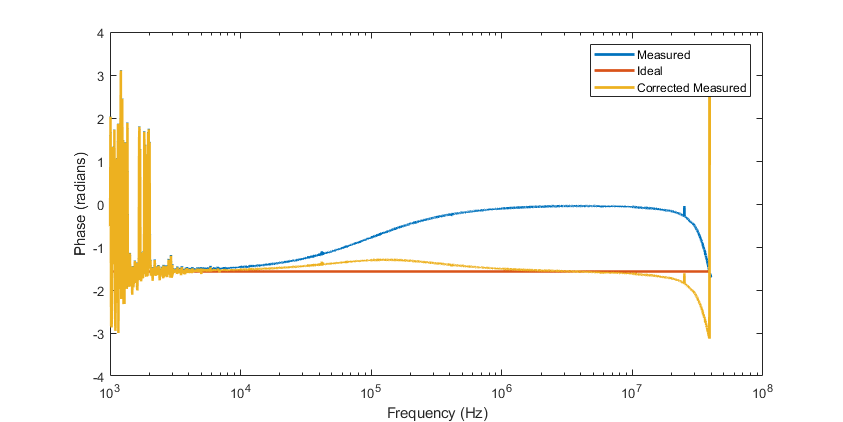
\includegraphics[width=\textwidth]{images/CorrectedImpedancePhase.png}
    \caption{Plot of the measured, ideal, and corrected measured impedance phase.}
\end{subfigure}
\caption{Impedance plot in polar form of the measured circuit, the ideal circuit, and the measured circuit with the applied correction function.}
\label{fig:IS_validation_corrected_spectra_comp}
\end{figure}

\begin{figure}[t]
    \centering
    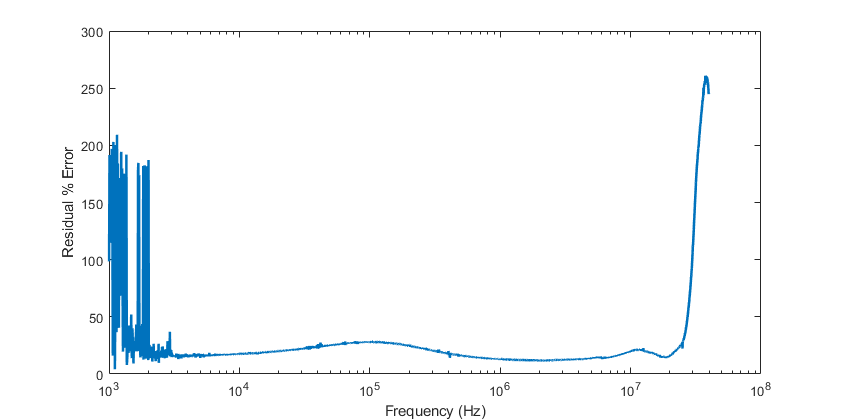
\includegraphics[width=\textwidth]{images/residualPercentError.png}
    \caption{Residual percent error of impedance spectra after applying the correction function. Between 3 kHz and 25 MHz, the residual error does not exceed 30$\%$.}
    \label{fig:IS_residual_error}
\end{figure}

\FloatBarrier


\subsection{Impedance Spectroscopy Reproducibility}

\par To characterize and assess the operation of the impedance spectroscopy chip, PBS medium samples were tested over the of three consecutive days to examine the reproducibility of the device, and deionized water, PBS medium, and PBS with 7 $\mu$m beads were tested to characterize device response to multiple solutions and to attempt a measurement of particles.

\par Figure \ref{fig:IS_data_reproducibility} displays the impedance spectra of PBS over three consecutive days and figure \ref{fig:IS_data_reproducibility_SD} shows the standard deviation of the sample set. Although a larger sample set covering more days would be desirable, the repeated impedance spectra behaviour and tight standard deviation imparts confidence of reproducibility.

\par With all the recorded data, signals became incoherent at low frequencies with high impedance loads. Data became , the data will gibberish the impedance magnitude will sometimes flatline, and 

\begin{figure}[h]
    \centering
    \begin{subfigure}[b]{\textwidth}
        \centering
        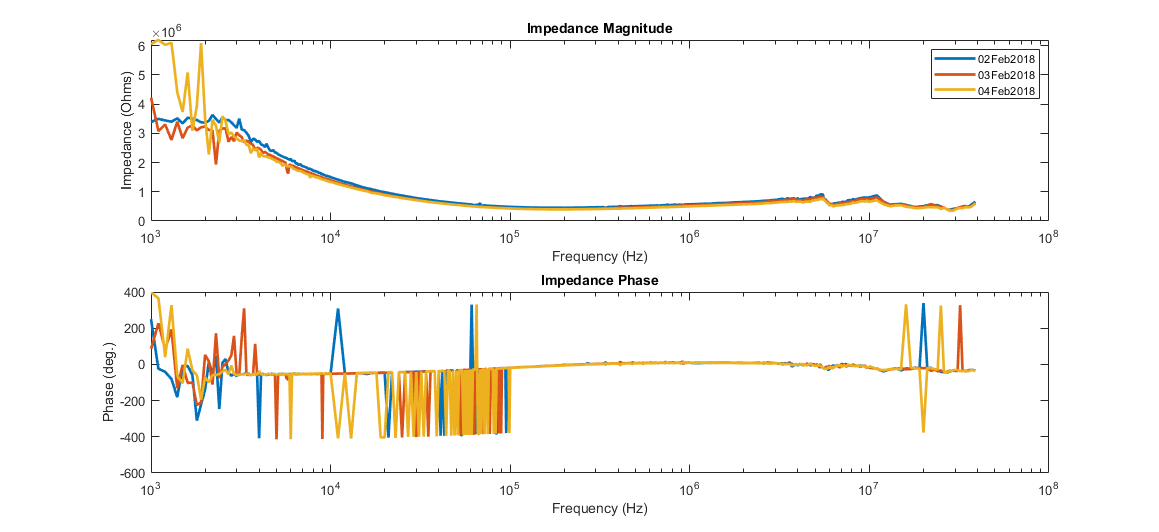
\includegraphics[width=\textwidth]{images/reproducibility_PBS_mag_phase.png}
        \caption{PBS impedance spectroscopy results in polar form.}
    \end{subfigure}
    \\
    \vspace{0.1 in}
    \begin{subfigure}[b]{\textwidth}
        \centering
        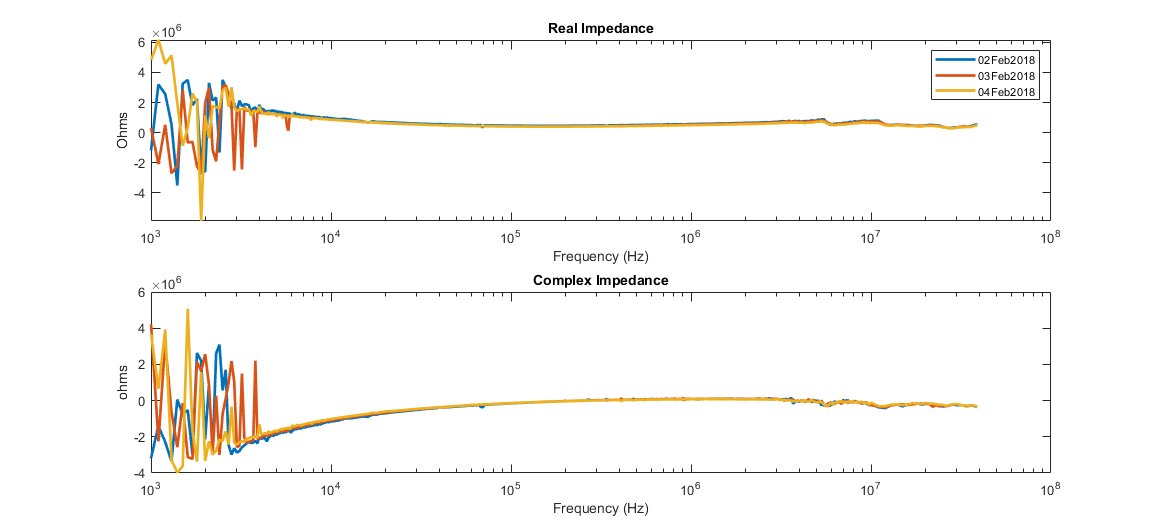
\includegraphics[width=\textwidth]{images/reproducibility_PBS_real_imag.png}
        \caption{PBS impedance spectroscopy results in rectangular form.}
    \end{subfigure}
    \caption{Reproducibility of the demonstrated with repeated measurement of phosphate buffered solution over a span of three days.}
    \label{fig:IS_data_reproducibility}
\end{figure}

\begin{figure}[h]
    \centering
    \begin{subfigure}[b]{\textwidth}
        \centering
        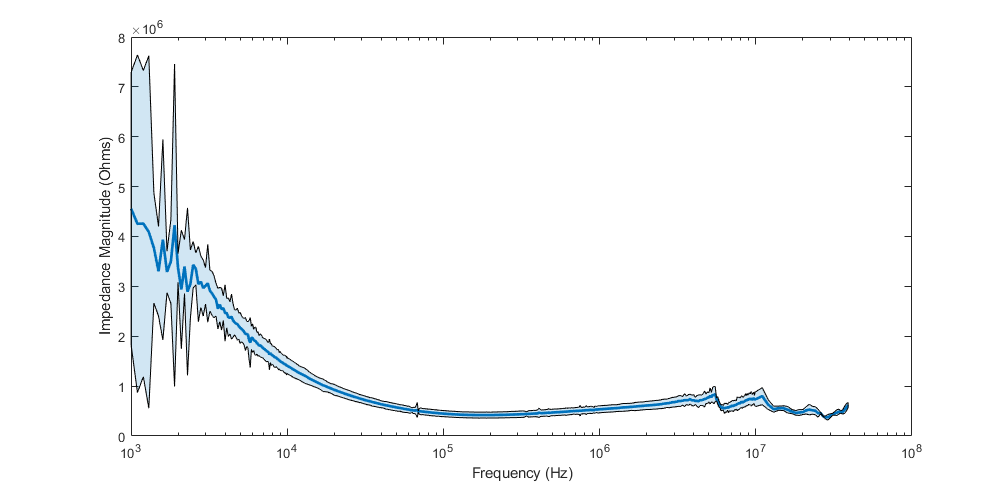
\includegraphics[width=\textwidth]{images/reproducibility_mean_std.png}
        \caption{The mean and 2x standard deviation of the impedance magnitude of the repeatability studies.}
    \end{subfigure}
    \\
    \vspace{0.1 in}
    \begin{subfigure}[b]{\textwidth}
        \centering
        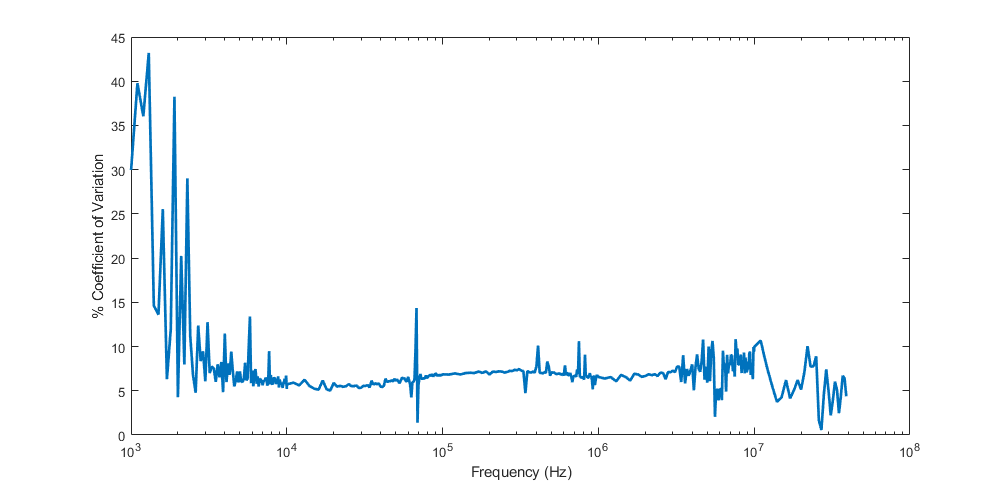
\includegraphics[width=\textwidth]{images/reproducibility_CV.png}
        \caption{The \% coefficient of variation of the impedance magnitude calculated from the repeatability studies.}
    \end{subfigure}
    \caption{Measured variability of the repeatability studies expressed as the standard deviation and the coefficient of variation.}
    \label{fig:IS_data_variation}
\end{figure}


\subsection{Impedance Spectroscopy Performance}

\par Impedance spectra for DI water, PBS, and 7 $\mu$m beads suspended in PBS were acquired and representive samples are displayed in figure \ref{fig:IS_data_beads_pbs_DI_comp}. The collected data met the expectations set by the material properties (NOTE: include table of material properties somewhere. methods? intro?). Deionized water exhibited the highest impedance with its low conductance, the conductive PBS responded with a significantly lower impedance, and the polystyrene beads suspended in PBS exhibited a larger capacitive load than the PBS by itself. However, as mentioned in the reproducibility study, low-frequency-high impedance loads continued to generate nonsense results and limit our viable frequency range.

\par In an attempt to isolate the effect of suspended polystyren beads in the PBS solution, the raw phase data was corrected, and the real and imaginary impedance spectra was recalculated, and then the difference between pbs-bead suspension and the pbs solution was calculated. The results are depicted in figure \ref{fig:clean_IS_data_beads_PBS_DI_comp}.

\begin{figure}[h]
    \centering
    \begin{subfigure}[b]{\textwidth}
        \centering
        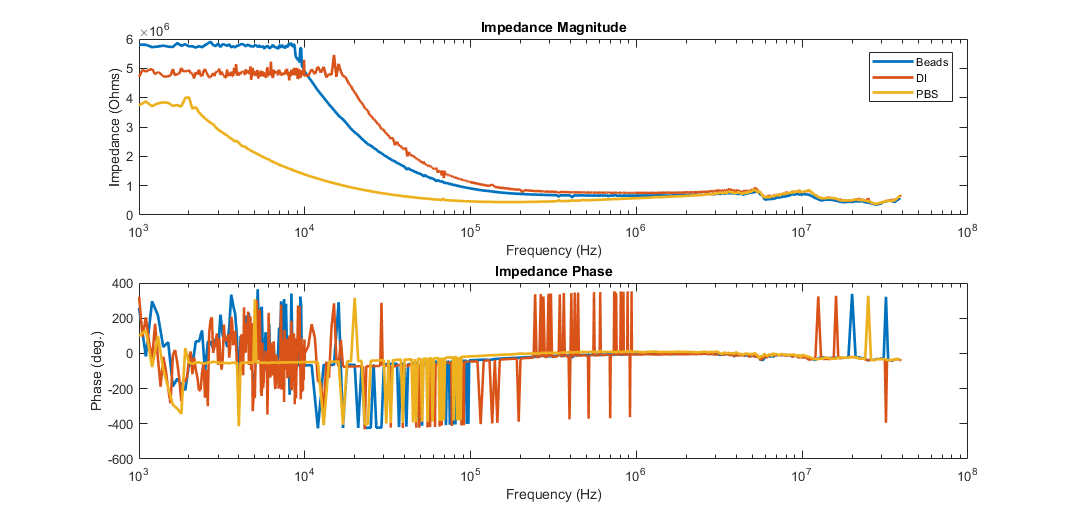
\includegraphics[width=\textwidth]{images/raw_IS_data_mag_phase.png}
        \caption{Impedance spectroscopy results in polar form.}
    \end{subfigure}
    \\
    \vspace{0.1 in}
    \begin{subfigure}[b]{\textwidth}
        \centering
        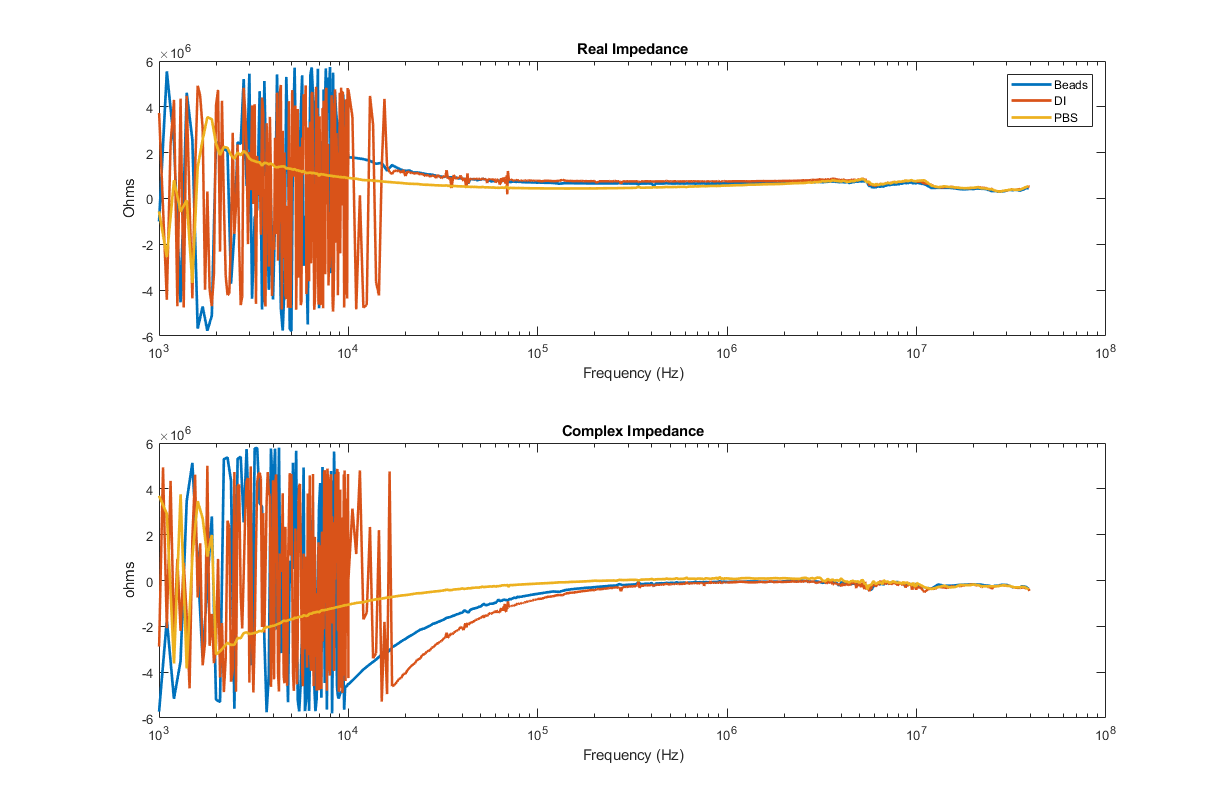
\includegraphics[width=\textwidth]{images/raw_IS_data_real_imag.png}
        \caption{Impedance spectroscopy results in rectangular form.}
    \end{subfigure}
    \\
%    \vspace{0.1 in}
%    \begin{subfigure}[b]{\textwidth}
%        \centering
%        \includegraphics[width=\textwidth]{images/raw_IS_%data_nyquist.png}
%        \caption{Jammed}
%    \end{subfigure}
    \caption[PBS, DI, microbead IS Raw data comparison.]{Comparison of impedance spectroscopy results using raw measurements of phosphate buffered solution, de-ionized water, and the chamber saturated with 7 $\mu$m polystyrene beads suspended in PBS.}
    \label{fig:IS_data_beads_pbs_DI_comp}
\end{figure}

\begin{figure}[h]
    \centering
    \begin{subfigure}[b]{\textwidth}
        \centering
        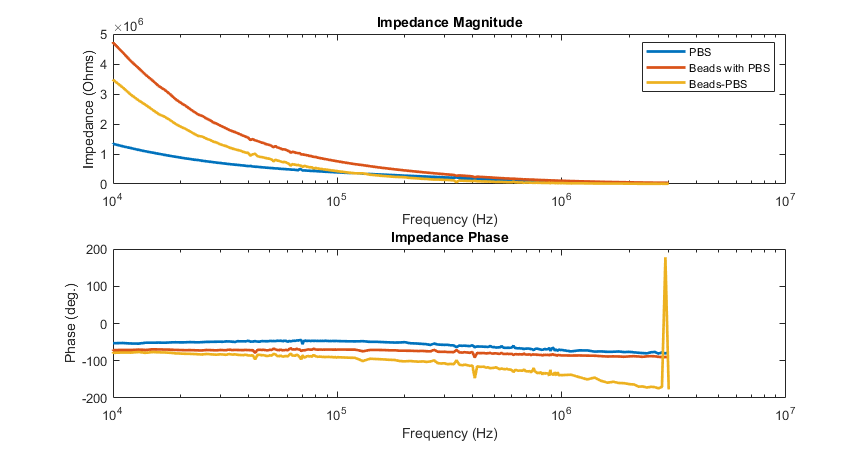
\includegraphics[width=\textwidth]{images/correctedPolar.png}
        \caption{IS results in polar form.}
    \end{subfigure}
    \\
    \vspace{0.1 in}
    \begin{subfigure}[b]{\textwidth}
        \centering
        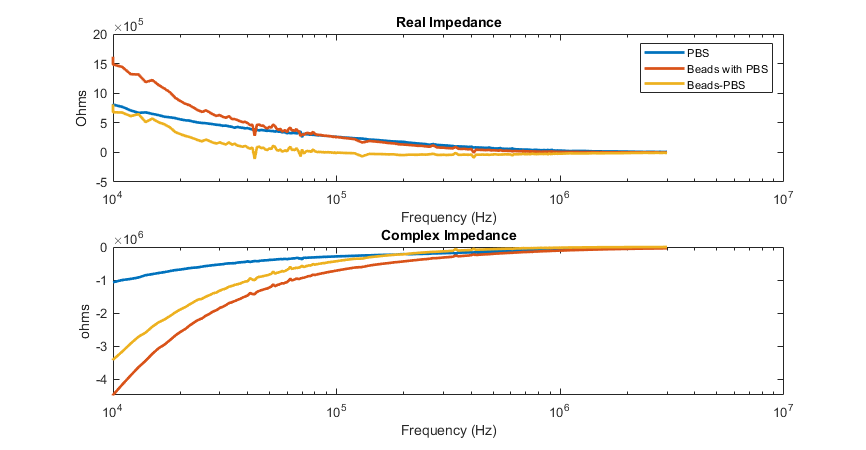
\includegraphics[width=\textwidth]{images/correctedRectangular.png}
        \caption{IS results in rectangular form.}
        \label{fig:clean_IS_data_beads_PBS_DI_comp}
    \end{subfigure}
    \\
    \vspace{0.1 in}
    %\begin{subfigure}[b]{\textwidth}
    %    \centering
    %    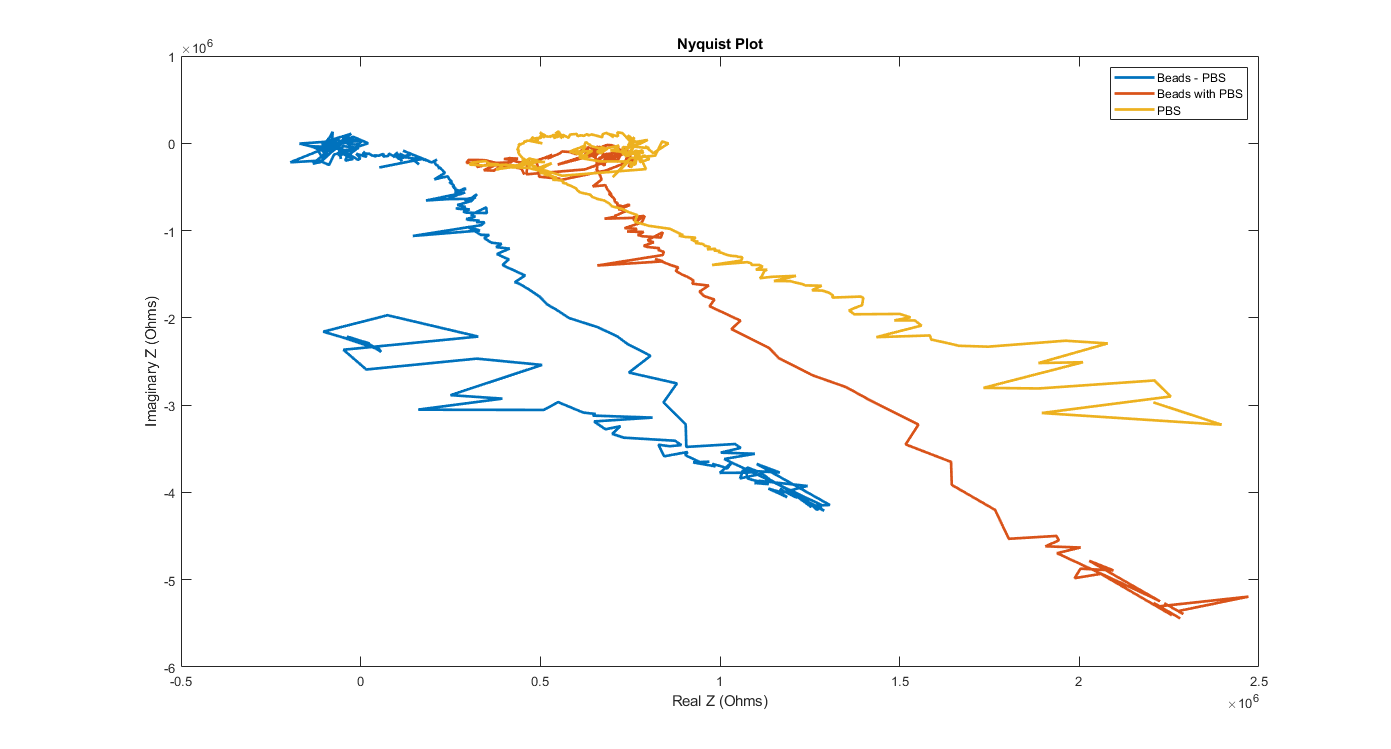
\includegraphics[width=\textwidth]{images/IS_data_clean_nyquist.png}
    %    \caption{Jammed}
    %\end{subfigure}
    \caption[PBS, PBS saturated with micro-beads, and the phasor difference.]{Comparison of impedance spectroscopy results from measurements of phosphate buffered solution, phosphate buffered solution saturated with 7 $\mu$m polystyrene beads, and the phasor difference between the two. The phase data was cleaned and the real and imaginary impedance was re-calculated.}
    \label{fig:IS_data_pbs_pbsBeads_difference}
\end{figure}

\par NOTE: Should include simulation to match empirical IS results.

\par NOTE: Consider rearranging order of results. Device fabrication -> IS DAQ validation -> Modeling -> Impedance Spectroscopy results -> simulations to match results (If possible)

%\begin{figure}[h]
%    \centering
%    \begin{subfigure}[b]{\textwidth}
%        \centering
%        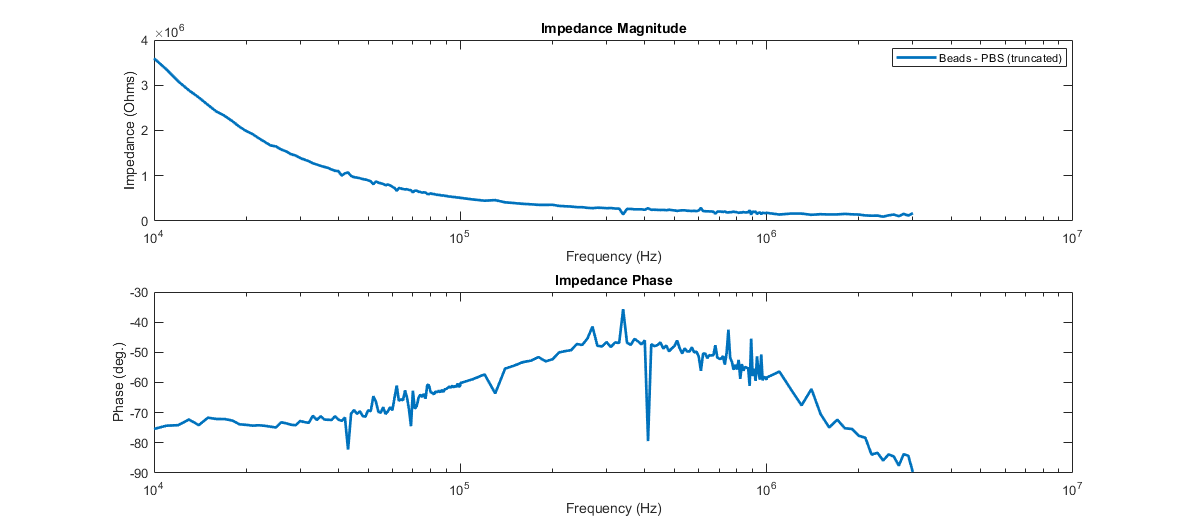
\includegraphics[width=\textwidth]{images/IS_data_beads-PBS_truncated_mag_phase.png}
%        \caption{Impedance spectra phasor difference in polar form.}
%    \end{subfigure}
%    \\
%    \vspace{0.1 in}
%    \begin{subfigure}[b]{\textwidth}
%        \centering
%        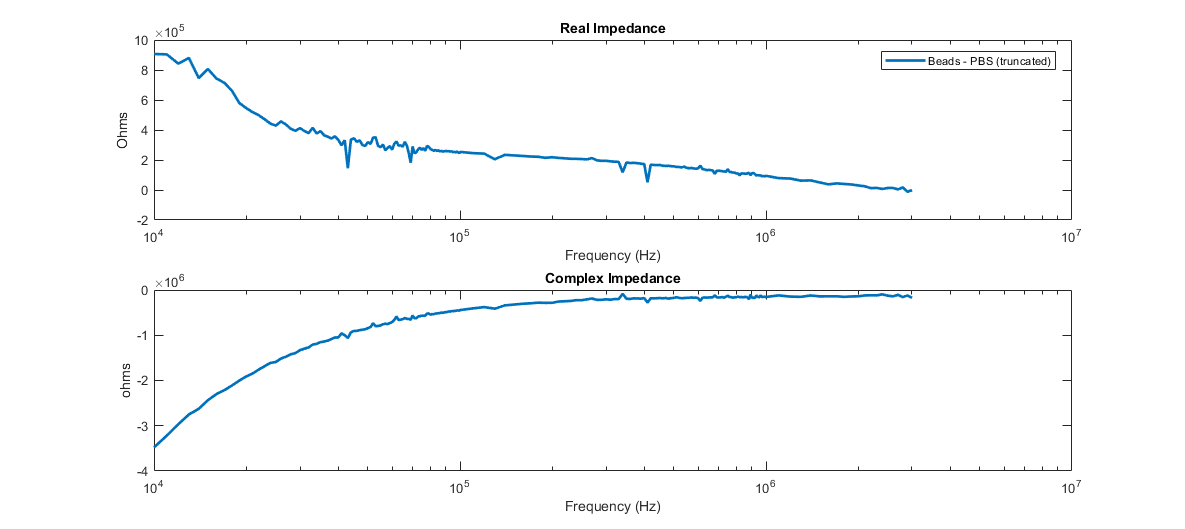
\includegraphics[width=\textwidth]{images/IS_data_beads-PBS_truncated_real_imag.png}
%        \caption{Impedance spectra phasor difference in rectangular form.}
%    \end{subfigure}
%    \\
    %\vspace{0.1 in}
    %\begin{subfigure}[b]{\textwidth}
    %    \centering
    %    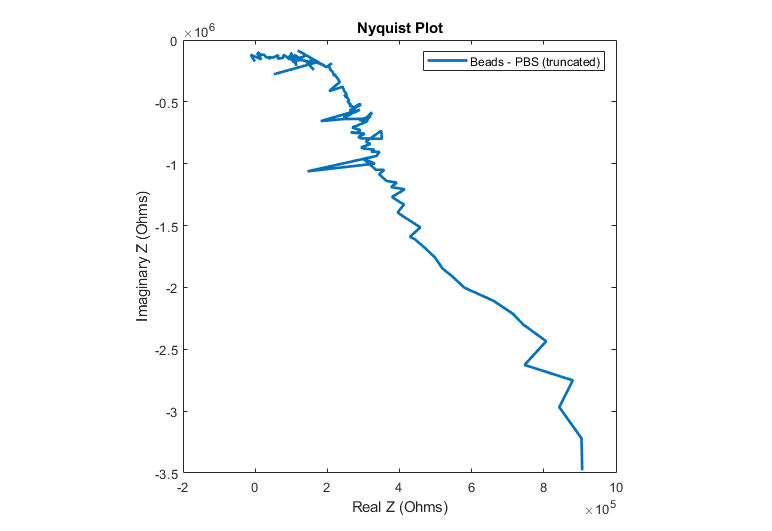
\includegraphics[width=\textwidth]{images/IS_data_beads-PBS_nyquist.png}
    %    \caption{Jammed}
    %\end{subfigure}
%    \caption[Truncated phasor difference between PBS, and micro-bead saturated PBS.]{Phasor difference between the PBS solution, and PBS solution saturated with 7$\mu$m microbeads. The data was truncated to the reliable frequency range of $10^4$ to $3$x$10^6$ hz.}
%    \label{fig:IS_data_beads_pbs_DI_comp}
%\end{figure}



\FloatBarrier

\subsection{Corrected Impedance Spectra}

\FloatBarrier

\section{Modeling}

\subsection{Impedance Spectroscopy Results}

\par Impedance response for the analytic solution, the simple FEA model, and the device model were calculated for medium saturation and a single cell suspension. The analytic solution utilized the power volume fraction discussed in section \ref{sec:novelVolumeFraction}. For details on the material properties used see table \ref{tab:fea_materials}. Additional information on the analytic solution is available in section \ref{sec:maxwell_mixture_theory} and details on the FEA model are available in section \ref{sec: FEA}. 

\par The results for the medium impedance spectra are given in figure \ref{fig:medium_model_IS_data}.The medium impedance spectra behaves as resistor and capacitor elements in parallel with a single relaxation starting around 100 Mhz, which is governed by the medium dielectric properties. In practice, an additional relaxation, governed by the polarization at the electrode-medium inteface (i.e. the EDL), would occur and largely mask the medium and cell relaxations. For these simulations the electric double layer phenomenon was excluded and addressed separately.

\par By comparing the three model results depicted in figure \ref{fig:medium_model_IS_data}, it can be noted that the device model has a significantly smaller impedance response than the analytic solution and the simple FEA model. This difference can be attributed to geometry and will be further explored later in this section. In addition, the analytic and simple model spectra are nearly identical, as expected since they model identical geometries.

\begin{figure}[h]
    \centering
    \begin{subfigure}[b]{\textwidth}
        \centering
        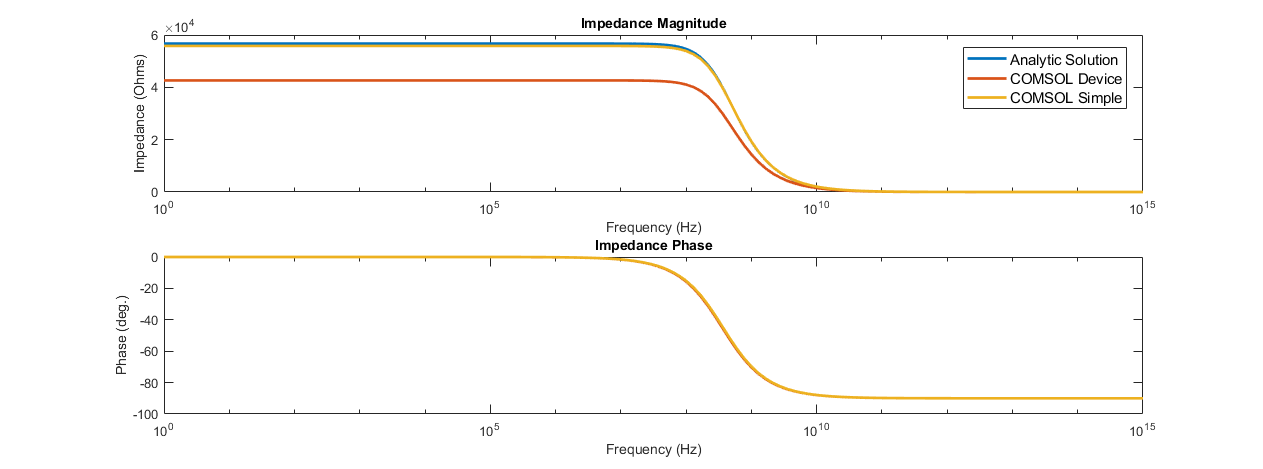
\includegraphics[width=\textwidth]{images/IS_model_medium_mag_phase.png}
        \caption{Impedance spectra in polar form.}
    \end{subfigure}
    \\
    \vspace{0.1 in}
    \begin{subfigure}[b]{\textwidth}
        \centering
        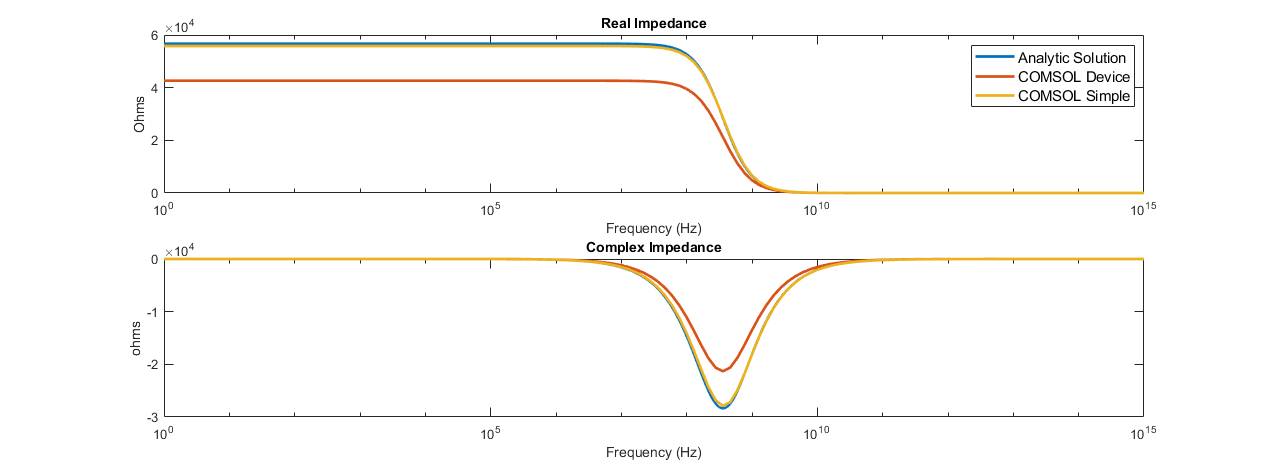
\includegraphics[width=\textwidth]{images/IS_model_medium_real_imag.png}
        \caption{Impedance spectra in rectangular form.}
    \end{subfigure}
    \\
    \vspace{0.1 in}
%    \begin{subfigure}[b]{\textwidth}
 %       \centering
  %      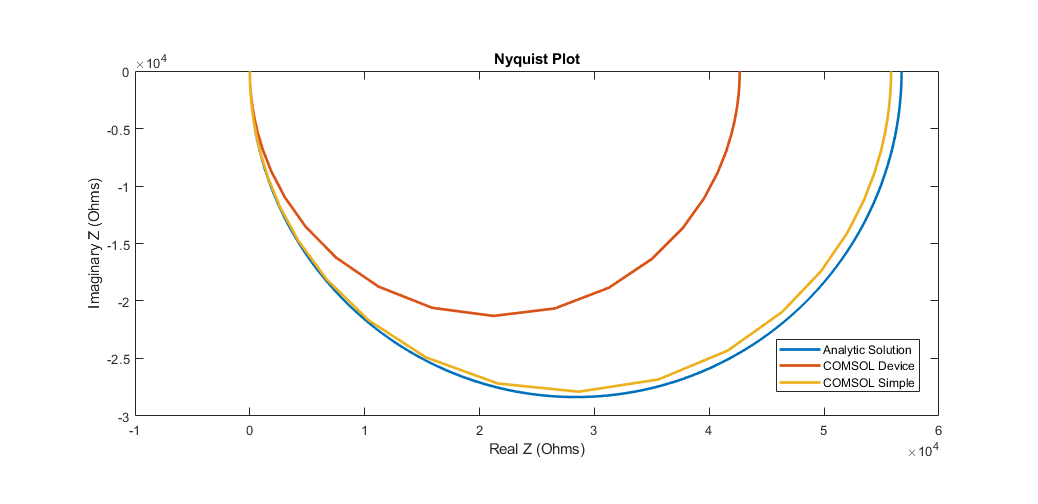
\includegraphics[width=\textwidth]{images/IS_model_medium_nyquist.png}
   %     \caption{Jammed}
    %\end{subfigure}
    \caption[Analyitic and FEA generated medium impedance spectrum]{Medium impedance spectrum generated by the analytic impedance solution, the simple FEA model, and the device FEA model.}
    \label{fig:medium_model_IS_data}
\end{figure}

\par With the inclusion of a single cell in the medium, the impedance spectra developed new dielectric dispersions. The simulated impedance spectra are depicted in figure \ref{fig:single_cell_model_IS_data}. According Pauly and Schwan, the addition of the single shelled cell into the system is expected to add two new relaxations to the impedance spectra: the Maxwell-Wagner relaxation that occurs from the polarization of the cell membrane with the medium, and the relaxation from polarization of the cytoplasm and medium at high frequencies when the cell membrane capacitance has been short-circuited \cit{paul&schwan},\cite{sun}. Refer to equations \ref{} and \ref{}, for the Pauly and Schwan description of these relaxations. The effect of the single cell is small, but can be readily identified as a small relaxation starting around 10 Mhz. However, the two distinct relaxations of the single shelled cell can't be distinguished among the large relaxation of the medium. The small size of the characteristic single cell suspension in comparison to the medium impedance spectrum highlights the importance of sensitivity optimization. The device model, which features a smaller device sensitivity, generated data with a significantly smaller relaxations due to the cell suspension. 

\begin{figure}[H]
    \centering
    \begin{subfigure}[b]{\textwidth}
        \centering
        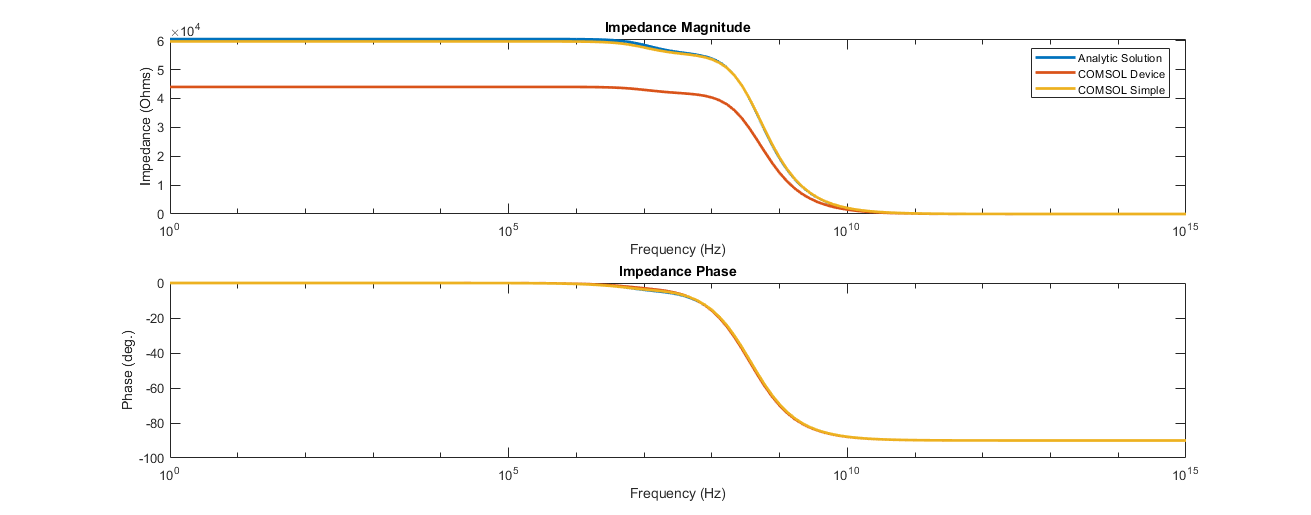
\includegraphics[width=\textwidth]{images/IS_model_mag_phase.png}
        \caption{Impedance spectra in polar form.}
    \end{subfigure}
    \\
    \vspace{0.1 in}
    \begin{subfigure}[b]{\textwidth}
        \centering
        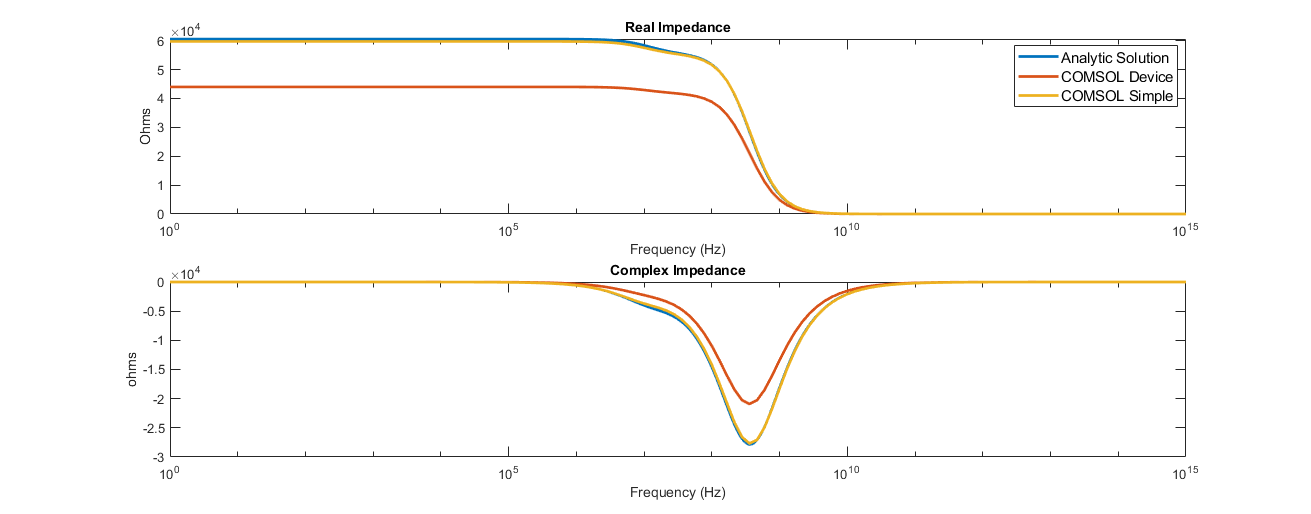
\includegraphics[width=\textwidth]{images/IS_model_real_imag.png}
        \caption{Impedance spectra in rectangular form.}
    \end{subfigure}
    %\\
    %\vspace{0.1 in}
    %\begin{subfigure}[b]{\textwidth}
      %  \centering
     %   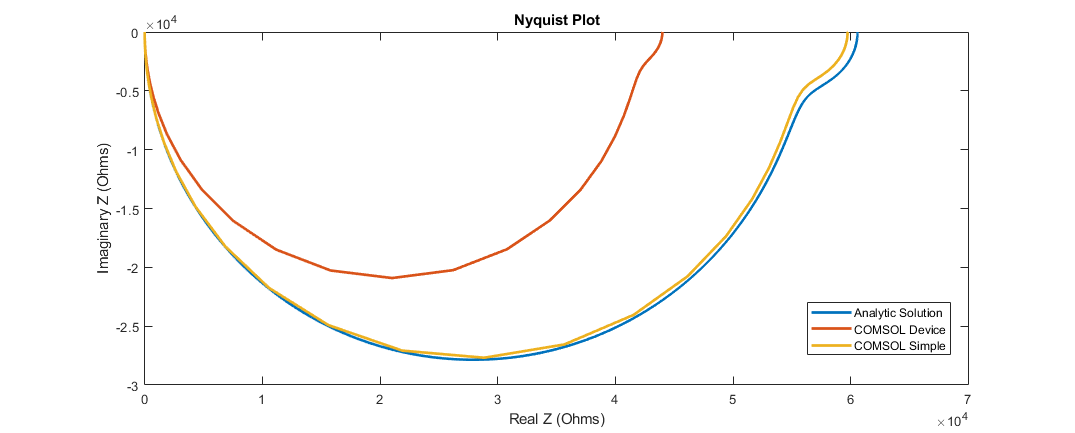
\includegraphics[width=\textwidth]{images/IS_model_nyquist.png}
%        \caption{Jammed}
%    \end{subfigure}
    \caption[Analyitic and FEA generated single cell impedance spectrums]{Single cell impedance spectrum generated by the analytic impedance solution, the simple FEA model, and the device FEA model.}
    \label{fig:single_cell_model_IS_data}
\end{figure}

%\begin{figure}[h]
%    \centering
%    \begin{subfigure}[b]{\textwidth}
%        \centering
%        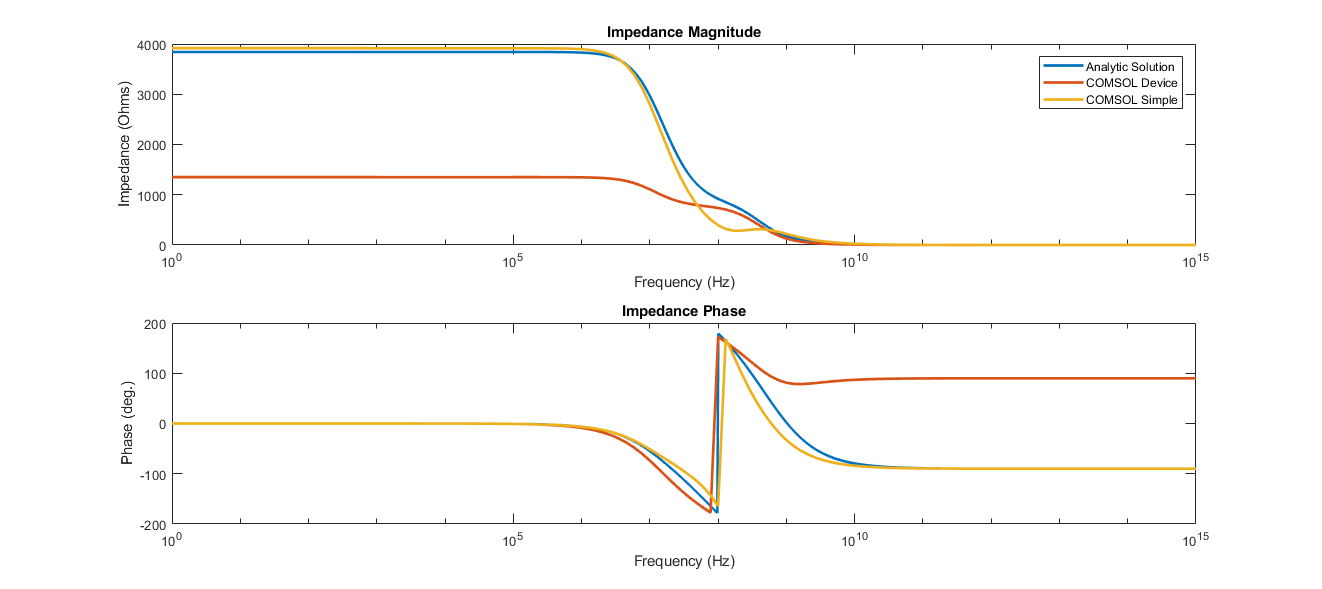
\includegraphics[width=\textwidth]{images/IS_model_difference_mag_phase.png}
%        \caption{Impedance spectra in polar form.}
%    \end{subfigure}
%    \\
%    \vspace{0.1 in}
%    \begin{subfigure}[b]{\textwidth}
%        \centering
%        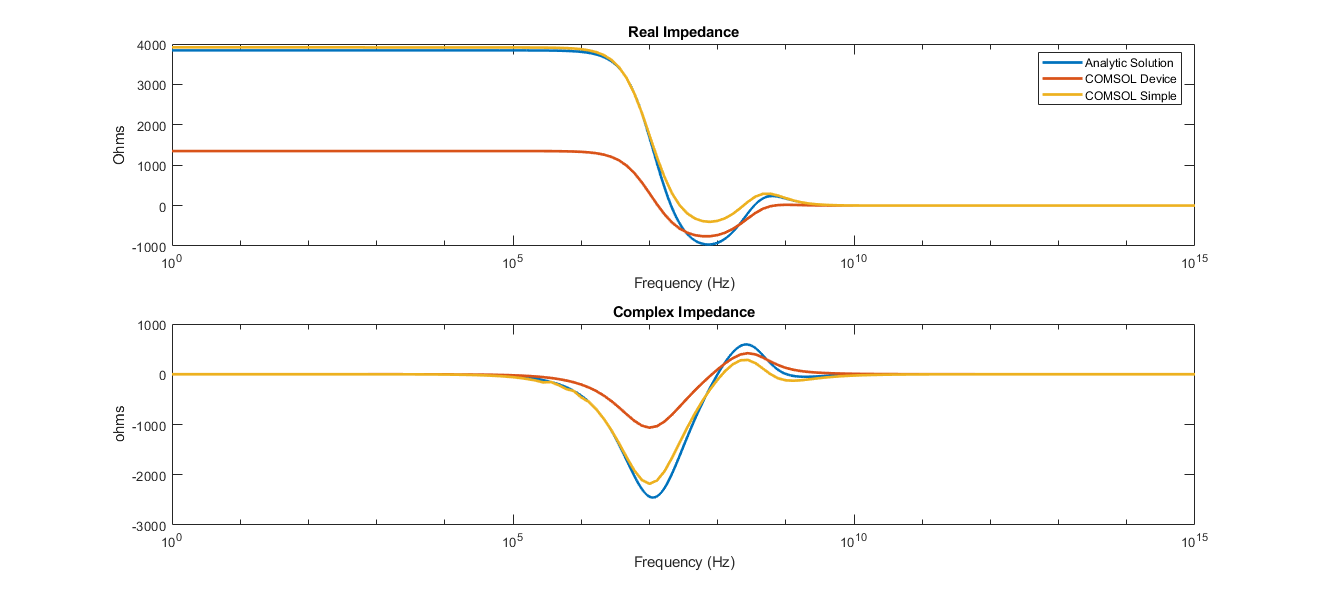
\includegraphics[width=\textwidth]{images/IS_model_difference_real_imag.png}
%        \caption{Impedance spectra in rectangular form.}
%    \end{subfigure}
%    \\
%    \vspace{0.1 in}
%    \begin{subfigure}[b]{\textwidth}
%        \centering
%        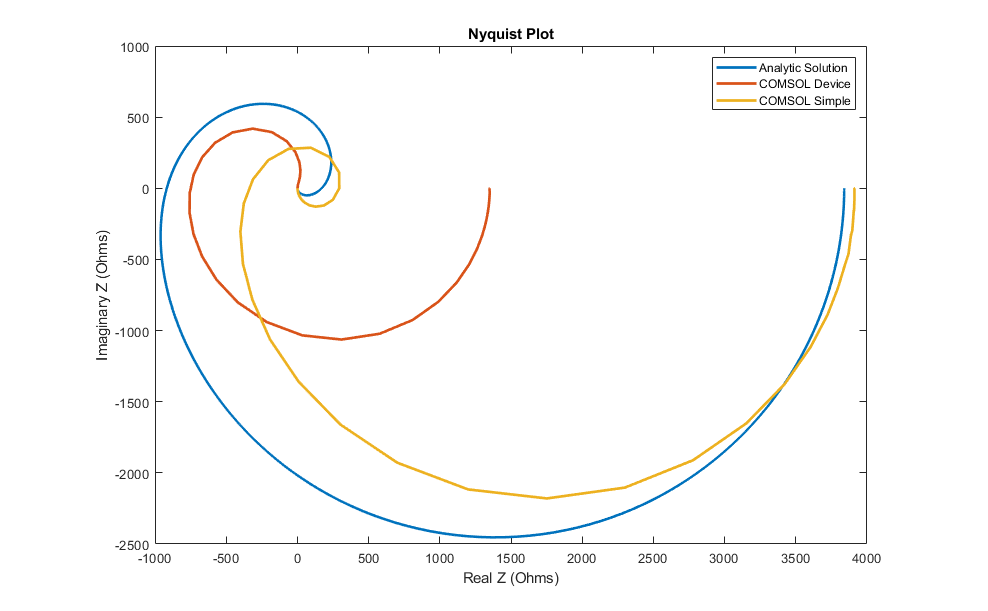
\includegraphics[width=\textwidth]{images/IS_model_difference_nyquist.png}
%        \caption{Jammed}
%    \end{subfigure}
%    \caption[Phasor difference between model mixture and medium impedance spectrum.]{Phasor difference between model mixture and medium impedance spectrum generated by the analytic impedance solution, the simple FEA model, and the device FEA model.}
%    \label{fig:single_cell_model_IS_data}
%\end{figure}

\begin{figure}[t!]
    \centering
    \begin{subfigure}[b]{\textwidth}
        \centering
        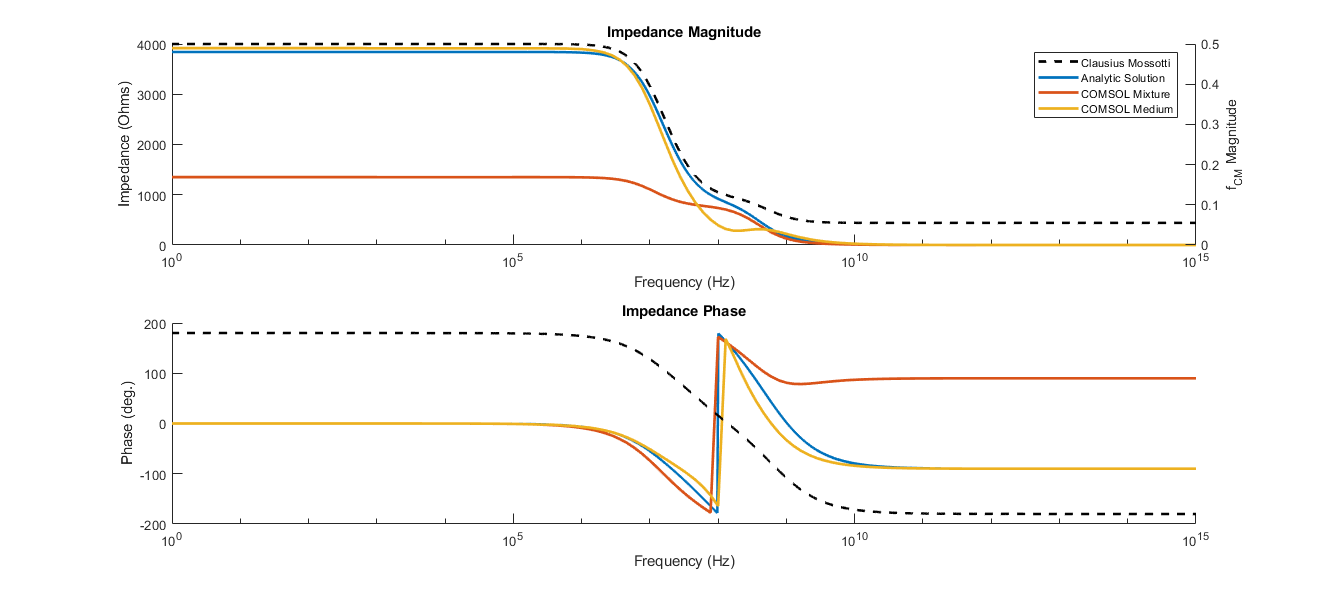
\includegraphics[width=\textwidth]{images/IS_model_difference_mag_phase_CM_overlay.png}
        \caption{Clausius Mossotti factor overlaid on difference impedance in polar form.}
        \label{fig:IS_model_difference_fcm_overlay_a}
    \end{subfigure}
    \\
    \vspace{0.1 in}
    \begin{subfigure}[b]{\textwidth}
        \centering
        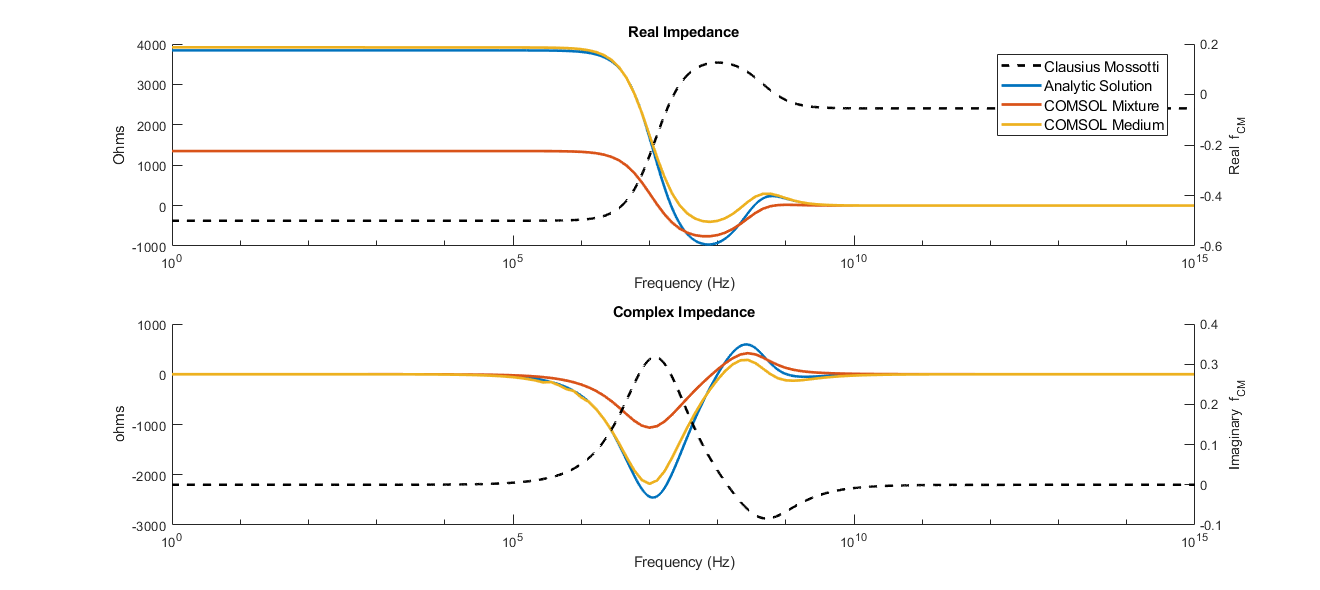
\includegraphics[width=\textwidth]{images/IS_model_real_imag_difference_CM_overlay.png}
        \caption{Clausius Mossotti factor overlaid on difference impedance in rectangular form.}
    \end{subfigure}

    \caption[Clausius Mossotti factor overlaid on IS model data.]{Clausius Mossotti factor overlaid on phasor difference between mixture and medium impedance spectrum model data generated from the analytic solution, the simple FEA model, and the device FEA model. It is clearly depicted how the impedance spectra tracks the Clausius Mossotti factor, and illustrates how the impedance responds to cell-medium dielectric dispersions.}
    \label{fig:IS_model_difference_fcm_overlay}
\end{figure}

\par To isolate the effect of the simulated cell, the difference between the single cell suspension and medium impedance spectra were generated and are displayed in figure \ref{fig:IS_model_difference_fcm_overlay}. The spectra in figure \ref{fig:IS_model_difference_fcm_overlay} are ideal results that could be obtained from using two differential sets of electrodes, where one pair measures the single cell suspension, and the second identical pair measures a chamber of only medium. This is a powerful configuration for bypassing the overbearing presence of the electric double layer in the impedance data and to distinguish the effects of the single cell. With the effects of the cell isolated the two characteristic cell relaxations can be easily identified near 10 MHz and 100 MHz.

\par In addition to the differential spectra, figure \ref{fig:IS_model_difference_fcm_overlay} also overlays the Clausius Mossotti factor. The Clausius Mossotti factor predicts the frequencies of dielectric dispersions, and can be used as a tool in system design and optimization. This application is further discussed in section \ref{sec:solution_optimization}.

\par As similarly noted in the medium and mixture impedance spectra results, the difference device impedance is significantly less pronounced. However, there are now discrepancies between the analytic solution and the simple FEA spectra. The differences begin to manifest at the onset of the Maxwell-Wagner relaxation at 10 MHz. Although the frequency positions of the dispersions coincide, the magnitude and shape of their spectra differ. This is most notable in the impedance magnitude chart in figure \ref{fig:IS_model_difference_fcm_overlay_a}. Since the analytic solution, device model, and the Clausius Mossotti spectra share the same shape, the simple model is suspected to contain errors. It is important to consider that FEA difference spectra are a small fraction of the impedance of the medium and mixture models from which it is derived, and that error can be magnified in the difference spectra. The simple FEA model should be revisited in future works.


\begin{figure}[H]
    \centering
    \includegraphics[width=0.7\textwidth]{images/deviceCellCurrent1Hz.png}
    \caption[Current density plot of the FEA device model.]{Current density plot of the FEA device model at DC. The color mapping depicts the logarithm of the current density magnitude.}
    \label{fig:device_current_denisty plot}
\end{figure}

\par One thing to note is the impedance magnitude for the device model is significantly smaller than the simple model. As depicted in figure \ref{fig:device_current_denisty plot}, it can be seen that the overlap of a flush channel and an electrode opens up an additional current path. To measure the designed device inefficiency, a surface integration of current density of the electrode region overlapping with the flush channel was calculated. 27.53\% and 29.29\% of the system current flowed through the flush channel electrode region without and with a cell in the sensor region respectively. The side channel inefficiency will effectively decrease the system cell constant and the effective volume fraction with the net effect of decreasing the device sensitivity.

\par To aid in visualizing how the impedance spectra develop as a function of frequency, figure \ref{fig:single_cell_model_EZ_plots} plots the electric field lines and magnitude of the center cross-section of the FEA simple model at characteristic frequencies.

\begin{figure}[h]
    \centering
    \begin{subfigure}[b]{\textwidth}
        \centering
        \includegraphics[width=\textwidth]{images/simple_cell_DC.png}
        \caption{The electric field at DC.}
    \end{subfigure}
    \\
    \vspace{0.1 in}
    \begin{subfigure}[b]{\textwidth}
        \centering
        \includegraphics[width=\textwidth]{images/simple_cell_1Mhz.png}
        \caption{The electric field at 1 Mhz. Need to consider where membrane and cytoplasm relaxation occurs}
    \end{subfigure}
    \\
    \vspace{0.1 in}
    \begin{subfigure}[b]{\textwidth}
        \centering
        \includegraphics[width=\textwidth]{images/simple_cell_10Mhz.png}
        \caption{The electric field magnitudes and isolines at 10 Mhz. The Maxwell-Wagner relaxation has taken affect as demonstrated by electric field line penetration of the cell.}
    \end{subfigure}
        \\
    \vspace{0.1 in}
    \begin{subfigure}[b]{\textwidth}
        \centering
        \includegraphics[width=\textwidth]{images/simple_cell_1Ghz.png}
        \caption{The electric field at 1 GHz.}
    \end{subfigure}
        \\
    \vspace{0.1 in}
    \begin{subfigure}[b]{\textwidth}
        \centering
        \includegraphics[width=\textwidth]{images/simpleCellColorMapAxis.png}
        \caption{The color map axis describing the magnitude of the electric field for the preceding sub-figures as log$_{10}(V/m)$.}
    \end{subfigure}
    \caption[FEA simple model electric field surface plot.]{FEA simple model plots of the electric field at frequencies of interest. The logarithm of the electric field magnitude is depicted through the color mapping outlined by the color axis in sub-figure (e), and the electric field lines are illustrated with white curves in the region of the electrodes and cell.}
    \label{fig:single_cell_model_EZ_plots}
\end{figure}


\FloatBarrier

\subsection{Solution Optimization}
\label{sec:solution_optimization}

\par An important take away from figure \ref{fig:IS_model_difference_fcm_overlay} is at what locations dielectric dispersions and Maxwell relaxation is occuring. For the parameters chosen in our single cell impedance spectroscopy models, dielectric relaxations occur above 40 MHz, the high frequency limit of our current impedance spectroscopy system. This is a strong impetus for us to revisit our IS DAQ and increase our operational frequency limit. There is another solution, albeit its flexibility is severely limited: changing the properties of the medium. The driving parameters in Clausius Mossotti factor are the dielectric properties of the medium and the particle. Given that we are to determine to measure said particle, that leaves us with altering the medium properties. Figure \ref{fig:FCM at different mediums } and \ref{fig: maxwell-wagner relaxation} depict how the frequencies of interest change as a function of medium properties. However, this method may be limited (or even non-available) depending on the application and the sensitivity of the target particle to the surrounding medium. For instance, the use of a hypotonic solution could lead to the swelling or rupture of cells such as erythrocytes.

\par NOTE: Include charts for FCM with different mediums and chart for maxwell-wagner. Should ensure proper discussion and equations occur in modeling and/or background section


\subsection{Device Optimization}


\subsection*{FEA Sensitivity Curves}

\begin{figure}[h]
    \centering
    \begin{subfigure}[t]{0.49\textwidth}
        \centering
        \includegraphics[width=\textwidth]{images/comsol_simple_difference.png}
        \caption{Impedance difference curve.}
    \end{subfigure}
    \hfill
    \begin{subfigure}[t]{0.49\textwidth}
        \centering
        \includegraphics[width=\textwidth]{images/comsol_simple_sensitivity_surface.png}
        \caption{Impedance sensitivity curve.}
    \end{subfigure}
    \\
    \vspace{0.1 in}
    \begin{subfigure}[t]{0.49\textwidth}
        \centering
        \includegraphics[width=\textwidth]{images/comsol_simple_gapXsensitivity.png}
        \caption{Sensitivity vs. gap.}
    \end{subfigure}
    \hfill
    \begin{subfigure}[t]{0.49\textwidth}
        \centering
        \includegraphics[width=\textwidth]{images/comsol_simple_widthXsensitivity.png}
        \caption{Sensitivity vs. width.}
    \end{subfigure}
    \caption[Simple FEA model sensitivity]{Parametric study on device sensitivity using the Simple FEA model. The study varied the electrode width and gap from 5 $\mu$m to 15 $\mu$m and 1 $\mu$m to 10 $\mu$m respectively. The Simple FEA model held a channel height of 10 $\mu$m and a cell centered between the two electrodes with a center height of 5 $\mu$m. The sensitivity was calculated with equation \ref{eqn:Sun_sensitivity}. See section \ref{sec: FEA} for additional details on the Simple FEA model.} 
    \label{fig:simple_sensitivity}
\end{figure}

\par To optimize the geometry of the device, a parametric analysis based on the electrode gap and width were run on the simple and device FEA models at DC. For each model the electrode width and gap were varied from 5 $\mu$m 15 $\mu$m and 1 $\mu$m to 10 $\mu$m respectively. All other geometry remained unchanged. Further details on the FEA models can be found in section \ref{sec: FEA}.

\par To better understand the results, the parametric curves are presented as the difference between the medium and cell suspension impedance, the sensitivity as defined by Sun in equation \ref{eqn:Sun_sensitivity}, the sensitivity curve projected onto the sensitivity-electrode gap plane, and the sensitivity projected onto the sensitivity-electrode width plane. The parametric study of the simple and device FEA model are presented in figure \ref{fig:simple_sensitivity} and \ref{fig:device_sensitivity} respectively.

\par (better for the discussion?) The impedance difference plot was included to show that although there is a peak for the maximum sensitivity, the impedance difference plateaus to a maximum as the electrode gap increases. The impedance difference and Sun's sensitivity tell us two different things: where the sensitivity is a ratio of the difference impedance to the medium impedance, the simple difference impedance gives us insight into the amount of non-relative amount of signal is from the cell. Depending on designer's goal, it may make sense to maximize your signal instead of your sensitivity, or to find a mixture of the two. 

\par It should be noted that the sensitivity curve for the FEA models is significantly "noisier" than the difference curves. This is likely due to "mesh noise". COMSOL generates a new mesh for each simulation in the parametric study. What is referred to as "mesh noise" is the accumulation of effects on results caused by differences in meshes. The appearance of "mesh noise" is a clear signal that the meshing scheme needs to revisited, as the purpose of mesh refinement is to remove the effect of meshes from the model. In this case, the mesh refinement was limited by system running COMSOL, but is definitely an area of future improvement. The sensitivity curves appear noisier due to the magnification of mesh noise from the extra operation on the results.

\par Although the mesh noise for the device model is severe, two are apparent in both the simple and device model.

\par The electrode gap is optimized at ?? around 5 microns. An intuitive reason behind this optimal electrode gap becomes apparent by observing the impedance difference curve. The impedance difference increases with the impedance gap. This is because as the electrode gap increases, the power felt by the cell increases. Likewise, the actual affect of the electrode width appears to be small, but even appears to increase the sensitivity with increased width. By widening the electrodes we are decreasing the cell constant (i.e. allowing more current flow) while the channels that the current must flow through decreases, at least until a certain point where a limit appears to be reached when current flowing from the electrode extremities is met with very high resistance. However, if the electric double layer was included in the model, and modeled as distributed capacitance over the electrodes, the wider the electrode the better since increased surface area would increase the capacitance and thus decrease impedance contributed by the electric double layer. 
\par With a smaller electrode gap the, more current travels the small distance between the electrodes an

\begin{figure}[h]
    \centering
    \begin{subfigure}[b]{0.49\textwidth}
        \centering
        \includegraphics[width=\textwidth]{images/comsol_device_surface_difference.png}
        \caption{Difference}
    \end{subfigure}
    \hfill
    \begin{subfigure}[b]{0.49\textwidth}
        \centering
        \includegraphics[width=\textwidth]{images/comsol_device_surface_sensitivity.png}
        \caption{Sensitivity}
    \end{subfigure}
    \\
    \vspace{0.1 in}
    \begin{subfigure}[b]{0.49\textwidth}
        \centering
        \includegraphics[width=\textwidth]{images/comsol_device_gapXsensitivity.png}
        \caption{gap}
    \end{subfigure}
    \hfill
    \begin{subfigure}[b]{0.49\textwidth}
        \centering
        \includegraphics[width=\textwidth]{images/comsol_device_widthXsensitivity.png}
        \caption{width}
    \end{subfigure}
    \caption[Device sensitivity]{Device sensitivity}
    \label{fig:device_sensitivity}
\end{figure}

\par Figure \ref{fig:device_sensitivity_average} attempts to clarify the electrode and and width sensitivity trends by averaging over contour lines.

\begin{figure}[h]
    \centering
    \begin{subfigure}[b]{0.49\textwidth}
        \centering
        \includegraphics[width=\textwidth]{images/comsol_device_gapXsensitivity_aveError.png}
        \caption{Gap}
    \end{subfigure}
    \hfill
    \begin{subfigure}[b]{0.49\textwidth}
        \centering
        \includegraphics[width=\textwidth]{images/comsol_device_widthXsensitivity_aveError.png}
        \caption{Width}
    \end{subfigure}
    \caption[Device sensitivity average]{Device sensitivity average}
    \label{fig:device_sensitivity_average}
\end{figure}

\par Electrode optimization was further clarified by using the analytic impedance solution to generate a higher resolution difference and sensitivity curves within a small fraction of the time required to generate the FEA derived results. 

\par Without any mesh noise, the effect of electrode geometry on the device sensitivity is clear. 

\par As the electrode gap increases, the amount of power felt by the cell increases, although the benefit of the increasing electrode gap begins to taper off. At the same time, the amount of medium the current travels through increases with the electrode gap increase. The balance between where the tapering power of the cell balances with the steadily increasing power of the medium is the optimal electrode location.

\par Although we did find an optimal electrode geometry for the 

\par Taking into account the channel height, the smaller the channel height the better. More current is forced to travel 

\par However, the fails to answer several additional questions relating to device optimization:
\begin{itemize}
    \item Does cell location change the optimized geometry?
    \item Does chamber height change the optimized geometry?
    \item What are the limits of our sensitivity curve?
    \item What is the effect of the electric double layer on the sensitivity curve?
\end{itemize}

\par Due to the time-consuming nature of COMSOL and its time-consuming nature, these questions were further explored using the analytic impedance solution and our novel power fraction.

\FloatBarrier

\subsection{Analytic Solution Sensitivity Curves}

\par There are three main advantages to using the analytic impedance solution for optimization over finite element methods:

\begin{enumerate}
	\item significantly faster run time, allowing for far higher resolutions over far greater ranges.
	\item General solution that isolates the effect of the electrode out from more complicated geometries.
	\item No mesh noise. Parametric analysis does not bring in the effects of re-meshing and effectively removes the effect of mesh artifacts from the simulation.
\end{enumerate}

\par To validate the analytic parametric studies, the simple FEA model, the analytic sensitivity calculated with Sun's definition and the power fraction, and the power fraction used as a sensitivity metric. To explore device behaviour and optimization, the more efficient power fraction is used to significantly expand the domain of the sensitivity analysis by exploring increased ranges in electrode gap, electrode height, channel height, particle location, and particle size. 

\begin{figure}
    \centering
    \begin{subfigure}{0.49\textwidth}
        \centering
        \includegraphics[width=\textwidth]{images/SunVsSimpleSensitivity.png}
        \caption{}
    \end{subfigure}
    \hfill
    \begin{subfigure}{0.49\textwidth}
        \centering
        \includegraphics[width=\textwidth]{images/SunVsSimplePercentDiff.png}
        \caption{}
    \end{subfigure}
    \caption{Caption}
    \label{fig:sunVsSimpleSensitivity}
\end{figure}


\begin{figure}[h]
    \centering
    \begin{subfigure}[b]{0.49\textwidth}
        \centering
        \includegraphics[width=\textwidth]{images/analytic_difference.png}
        \caption{Difference}
    \end{subfigure}
    \hfill
    \begin{subfigure}[b]{0.49\textwidth}
        \centering
        \includegraphics[width=\textwidth]{images/analytic_sun_surface.png}
        \caption{Sensitivity}
    \end{subfigure}
    \\
    \vspace{0.1 in}
    \begin{subfigure}[b]{0.49\textwidth}
        \centering
        \includegraphics[width=\textwidth]{images/analytic_sun_gapXsensitivity.png}
        \caption{gap}
    \end{subfigure}
    \hfill
    \begin{subfigure}[b]{0.49\textwidth}
        \centering
        \includegraphics[width=\textwidth]{images/analytic_sun_widthXsensitivity.png}
        \caption{width}
    \end{subfigure}
    \caption[Analytic Sensitivity]{Analytic Sensitivity}
    \label{fig:analytic_sensitivity}
\end{figure}

\begin{figure}[h]
    \centering
    \begin{subfigure}[b]{0.49\textwidth}
        \centering
        \includegraphics[width=\textwidth]{images/analytic_sun_difference_expanded.png}
        \caption{Difference}
    \end{subfigure}
    \hfill
    \begin{subfigure}[b]{0.49\textwidth}
        \centering
        \includegraphics[width=\textwidth]{images/analytic_sun_surface_expanded.png}
        \caption{Sensitivity}
    \end{subfigure}
    \\
    \vspace{0.1 in}
    \begin{subfigure}[b]{0.49\textwidth}
        \centering
        \includegraphics[width=\textwidth]{images/analytic_sun_gapXsensitivity_extended.png}
        \caption{gap}
    \end{subfigure}
    \hfill
    \begin{subfigure}[b]{0.49\textwidth}
        \centering
        \includegraphics[width=\textwidth]{images/analytic_sun_widthXsensitivity_extended.png}
        \caption{width}
    \end{subfigure}
    \caption[Analytic Sensitivity]{Analytic Sensitivity}
    \label{fig:analytic_sensitivity}
\end{figure}

\begin{figure}[h]
    \centering
    \begin{subfigure}[b]{0.49\textwidth}
        \centering
        \includegraphics[width=\textwidth]{images/analytic_power_surface.png}
        \caption{Power Surface}
    \end{subfigure}
    \hfill
    \begin{subfigure}[b]{0.49\textwidth}
        \centering
        \includegraphics[width=\textwidth]{images/analytic_gapXpower.png}
        \caption{GapXpower by width}
    \end{subfigure}
    \\
    \vspace{0.1 in}
    \begin{subfigure}[b]{0.49\textwidth}
        \centering
        \includegraphics[width=\textwidth]{images/analytic_widthXpowerByHeight.png}
        \caption{width x power by height}
    \end{subfigure}
    \hfill
    \begin{subfigure}[b]{0.49\textwidth}
        \centering
        \includegraphics[width=\textwidth]{images/analytic_heightXpowerByGap.png}
        \caption{height x power by gap}
    \end{subfigure}
    \caption[power comp]{power comp}
    \label{fig:analytic_sensitivity}
\end{figure}


\begin{figure}[h]
    \centering
    \begin{subfigure}[b]{0.49\textwidth}
        \centering
        \includegraphics[width=\textwidth]{images/analytic_vertical_power.png}
        \caption{Power Surface}
    \end{subfigure}
    \hfill
    \begin{subfigure}[b]{0.49\textwidth}
        \centering
        \includegraphics[width=\textwidth]{images/analytic_horizontal_power.png}
        \caption{GapXpower by width}
    \end{subfigure}
    \\
    \vspace{0.1 in}
    \begin{subfigure}[b]{0.49\textwidth}
        \centering
        \includegraphics[width=\textwidth]{images/analytic_vertical_power_width20.png}
        \caption{width x power by height}
    \end{subfigure}
    \hfill
    \begin{subfigure}[b]{0.49\textwidth}
        \centering
        \includegraphics[width=\textwidth]{images/analytic_horizontal_power_20width.png}
        \caption{height x power by gap}
    \end{subfigure}
    \caption[power comp]{power comp}
    \label{fig:analytic_sensitivity}
\end{figure}

testing